\subsubsection{Tent map (TENT)} \label{sssec:tent}

The Tent map has been extensively studied in the literature because theoretically it has nice  statistical properties that can be analytically obtained. For example it is easy to proof that it has a uniform histogram and consequently an ideal $H_{hist}=1$. The Perron-Frobenius operator and its corresponding eigenvalues and eigenfunctions may be also be analytically obtained for this map \cite{tent}. 

This map is represented with the equation:
\begin{equation}\label{eq:tentmap}
x_{n+1}~=~ \left\{ \begin{array}{ll}
2~{x_n} & \textrm{if ~$0\leq x_n\leq 1/2$}\\
2~(1-{x_n}) & \textrm{if ~$1/2<x_n\leq 1$} 
\end{array} \right.  \ ,
\end{equation}
with $x_n\in\mathcal{R}$.

In Base-2 fractional numbers rounding, equation \ref{eq:tentmap} became
\begin{equation}\label{eq:tentdecbin}
x_{n+1}~=~ \left\{ \begin{array}{ll}
2~{x_n} & \textrm{if $0\leq x_n\leq 1/2$}\\
\epsilon \times floor\{\frac{2~-~2~x_n}{\epsilon}\} & \textrm{if $1/2<x_n\leq 1$} 
\end{array} \right.  \ ,
\end{equation}
with $\epsilon=2^{-B}$ for binary numbers.

When this map is implemented in a computer using any numerical representation system (even floating point!) truncation errors rapidly increases and makes the unstable fixed point in $x^*=0$ becomes stable producing a short transitory followed by an infinite number of  $0$'s\cite{Jessa1993,Callegari1997}.
This issue is easily explained in [with chaos meet computers], problem appears but all itarations has an shift-to-left operation that carry the $0's$ from right side.
Some authors \cite{buscar} have proposed to add a random perturbation to avoid this drawback of the Tent map. But this procedure introduces statistical properties of the random perturbation that are mixed with those of the Tent map itself.
Skew Tent is an option that allows reach nice statistical properties even in base 2 fractional numbers.
Here we study the Tent map "as it is" without any artifact to evaluate its real instead of theoretical statistical properties. 

Figs. \ref{fig:tent} (a) to (e) show the different quantifiers for floating point and fixed point numerical representation.
This map falls to $0$ in all cases with a short transitory between $0$ and $B$
Again $BPW$ quantifiers is diferent of $0$ because this procedure discards the elements once they reach the fixed point.
Because of this TENT map is not possible to use in 2-bassed computer.

\begin{figure}
	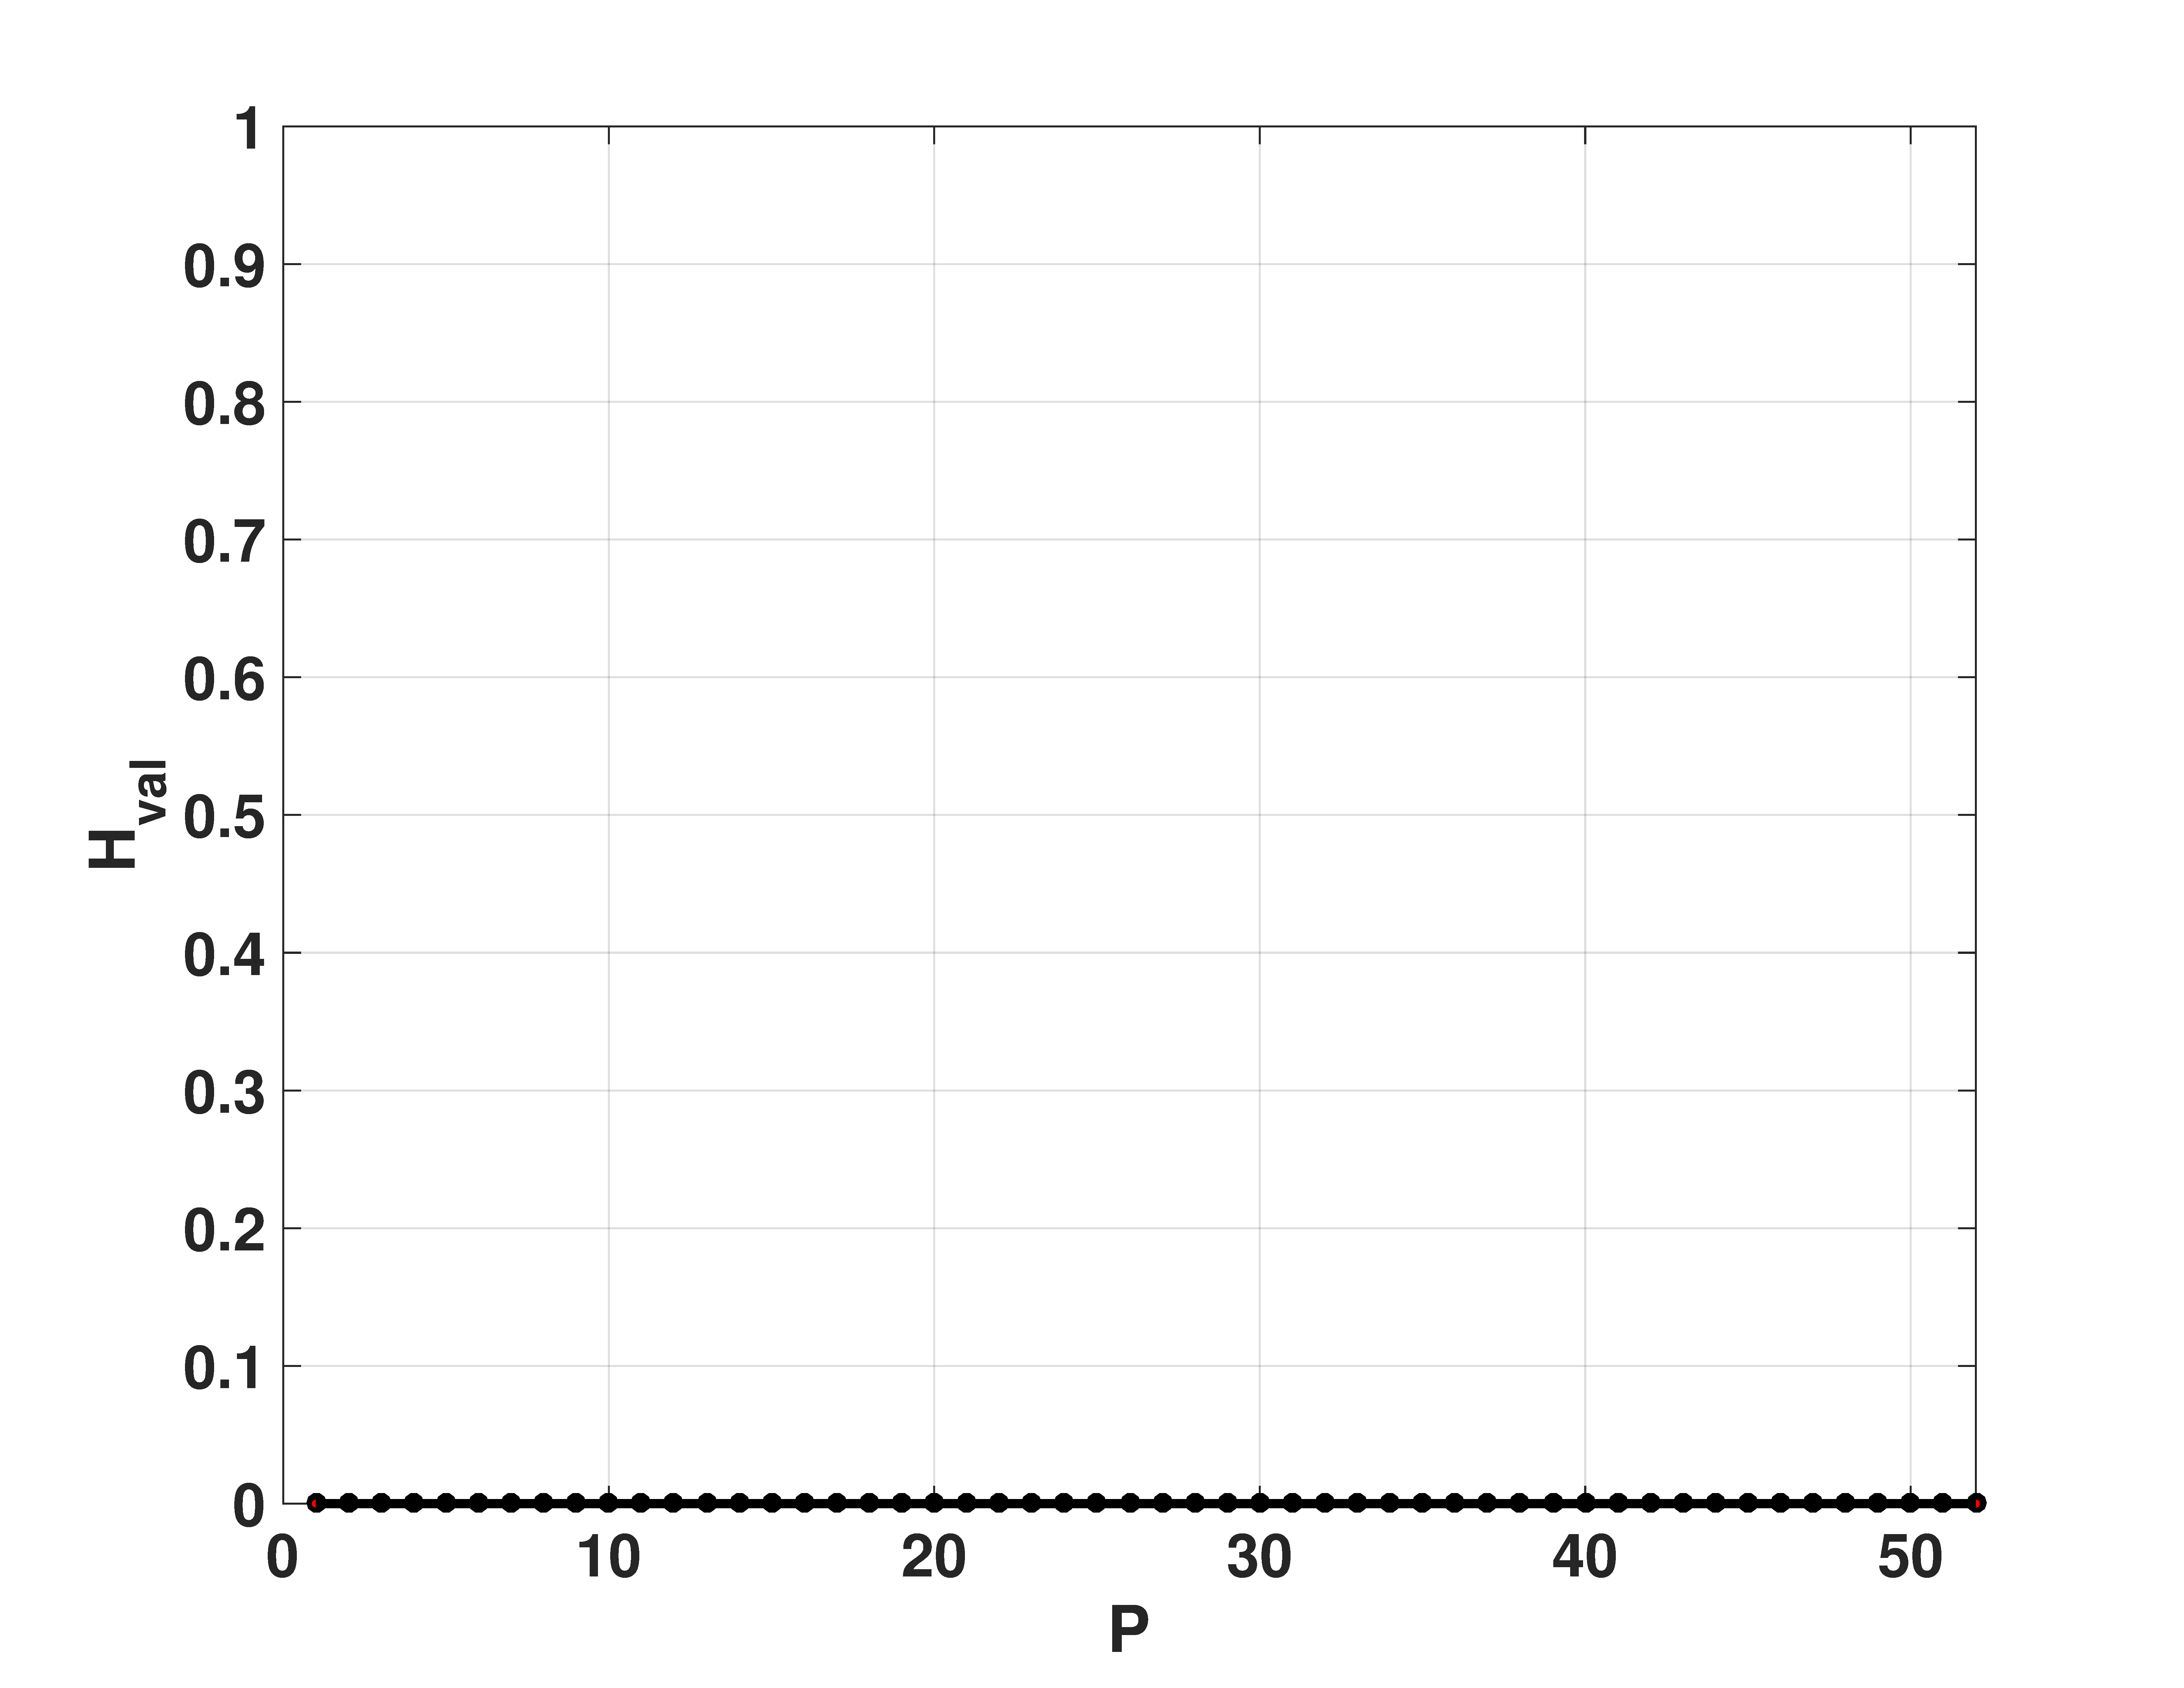
\includegraphics[width=.32\textwidth]{Hval_Tent}
	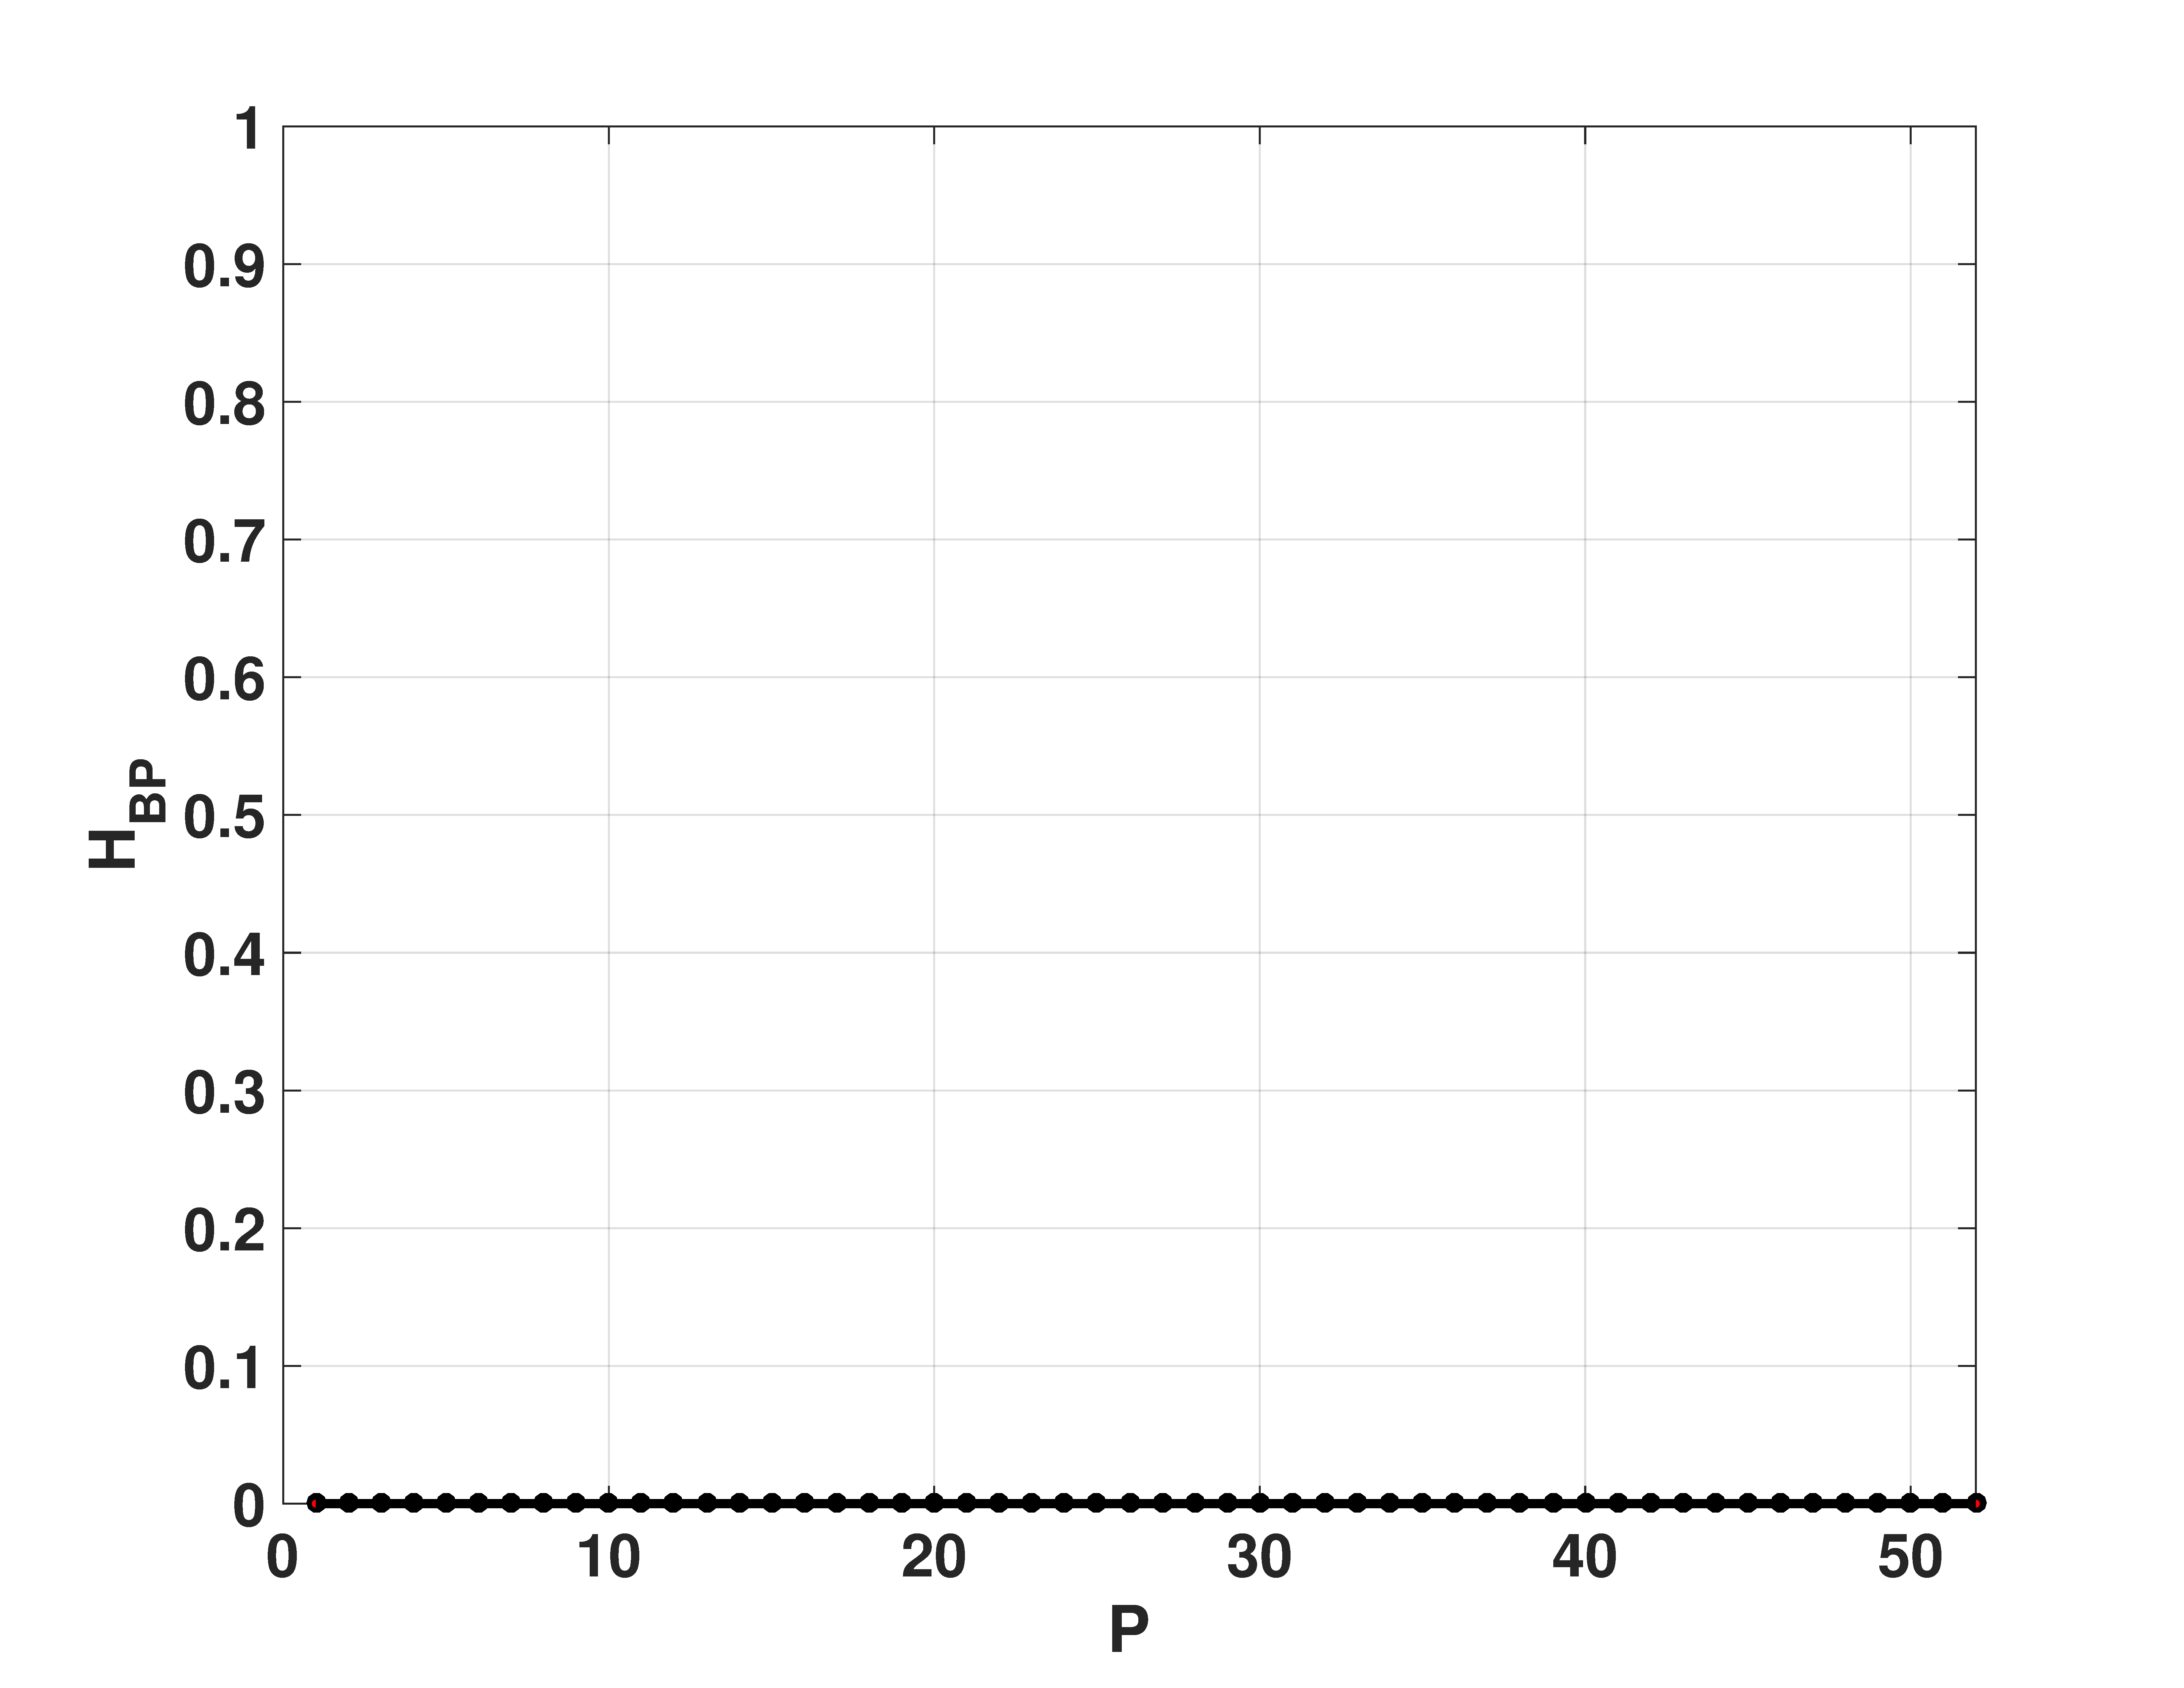
\includegraphics[width=.32\textwidth]{Hbp_Tent}
	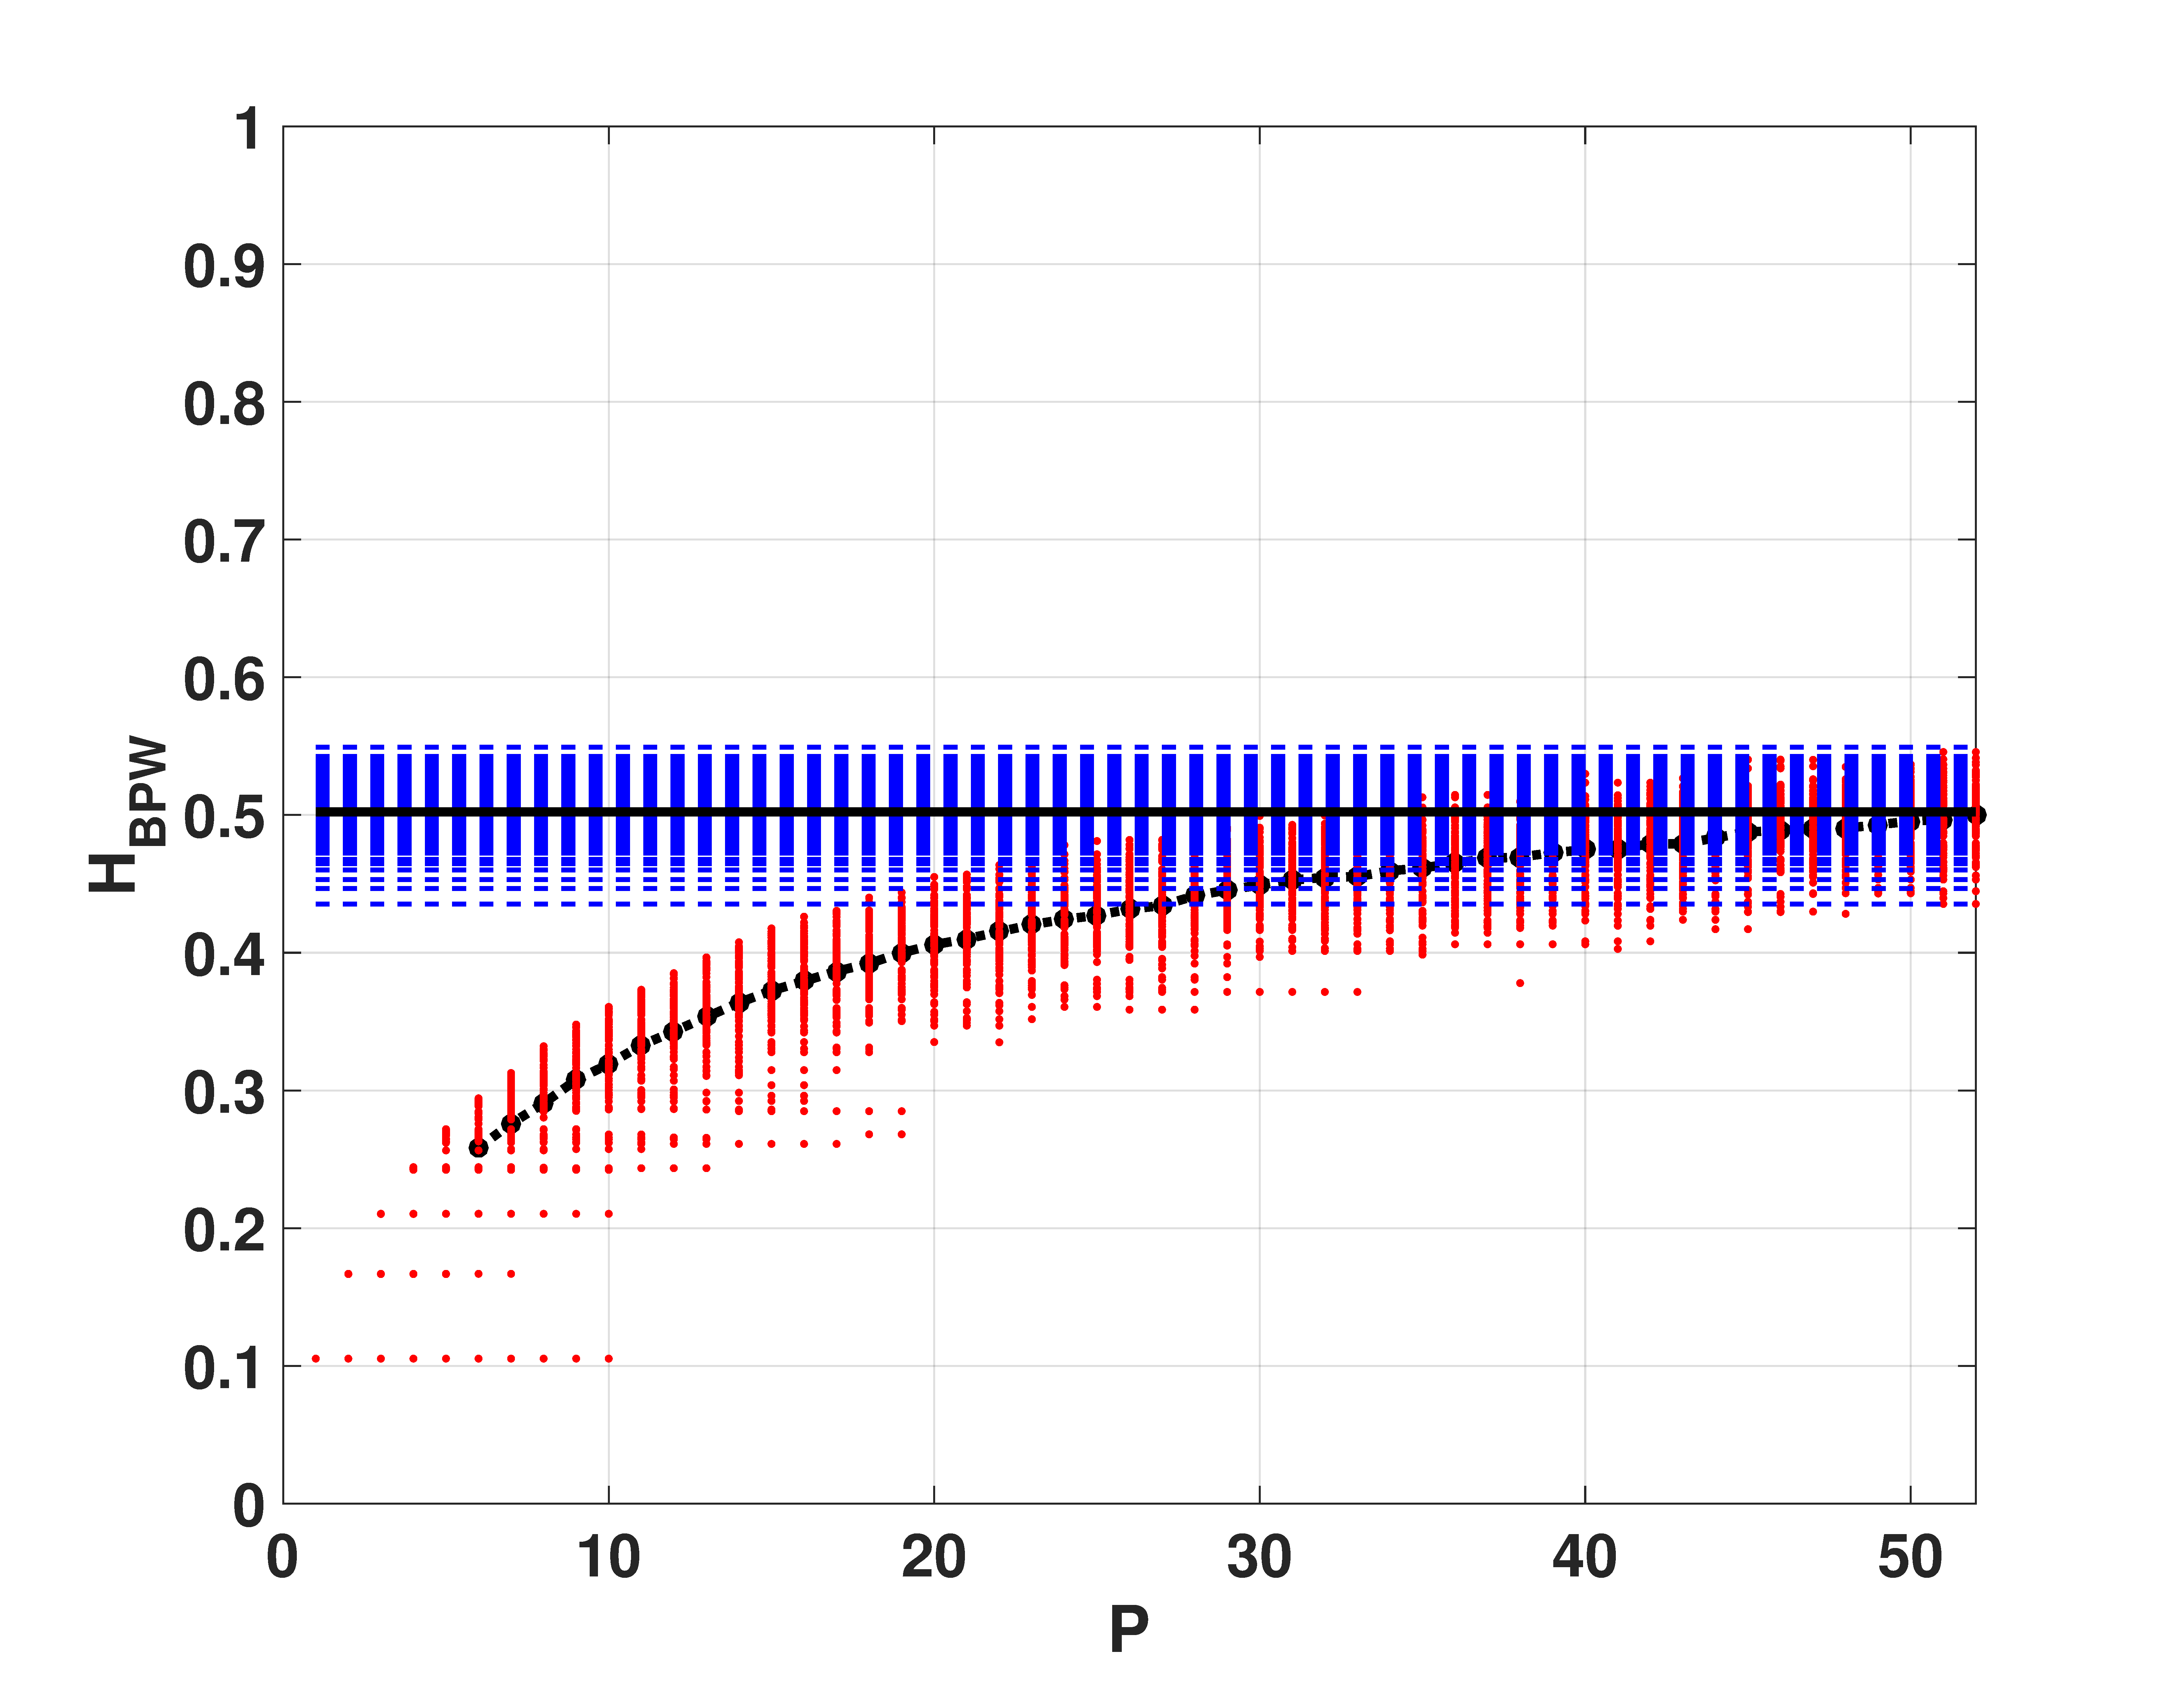
\includegraphics[width=.32\textwidth]{Hbpw_Tent}
	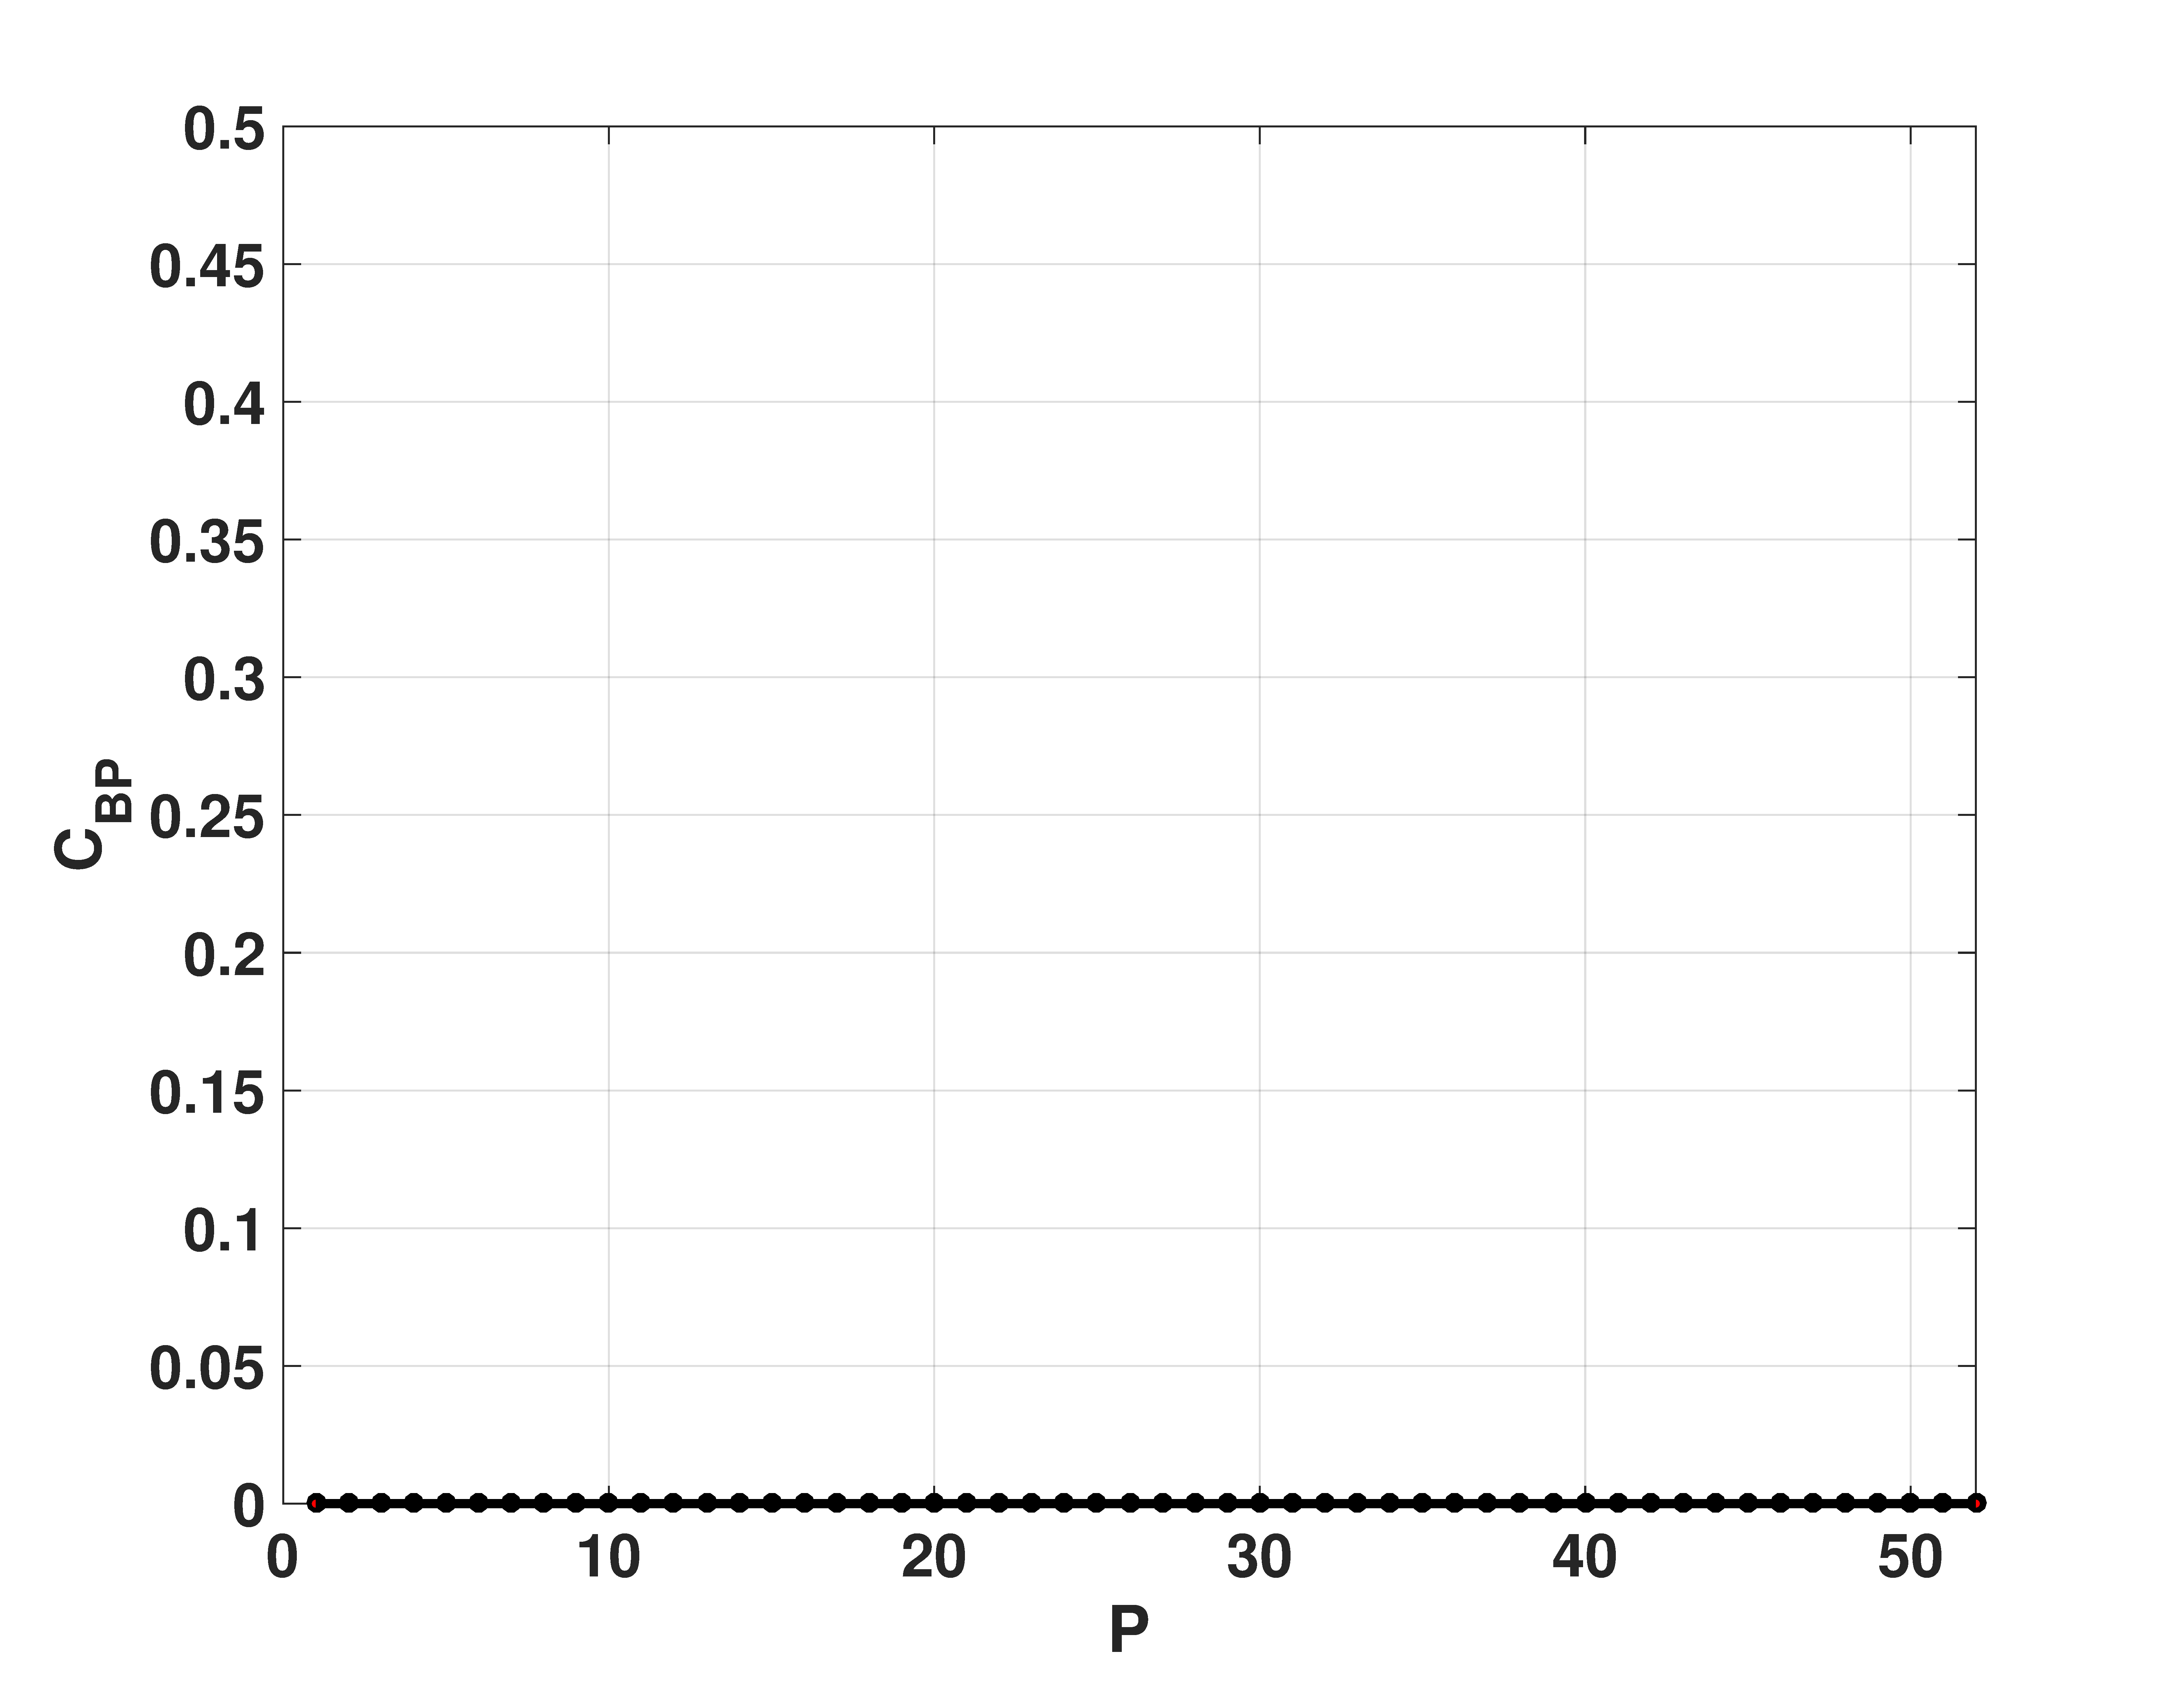
\includegraphics[width=.32\textwidth]{Cbp_Tent}
	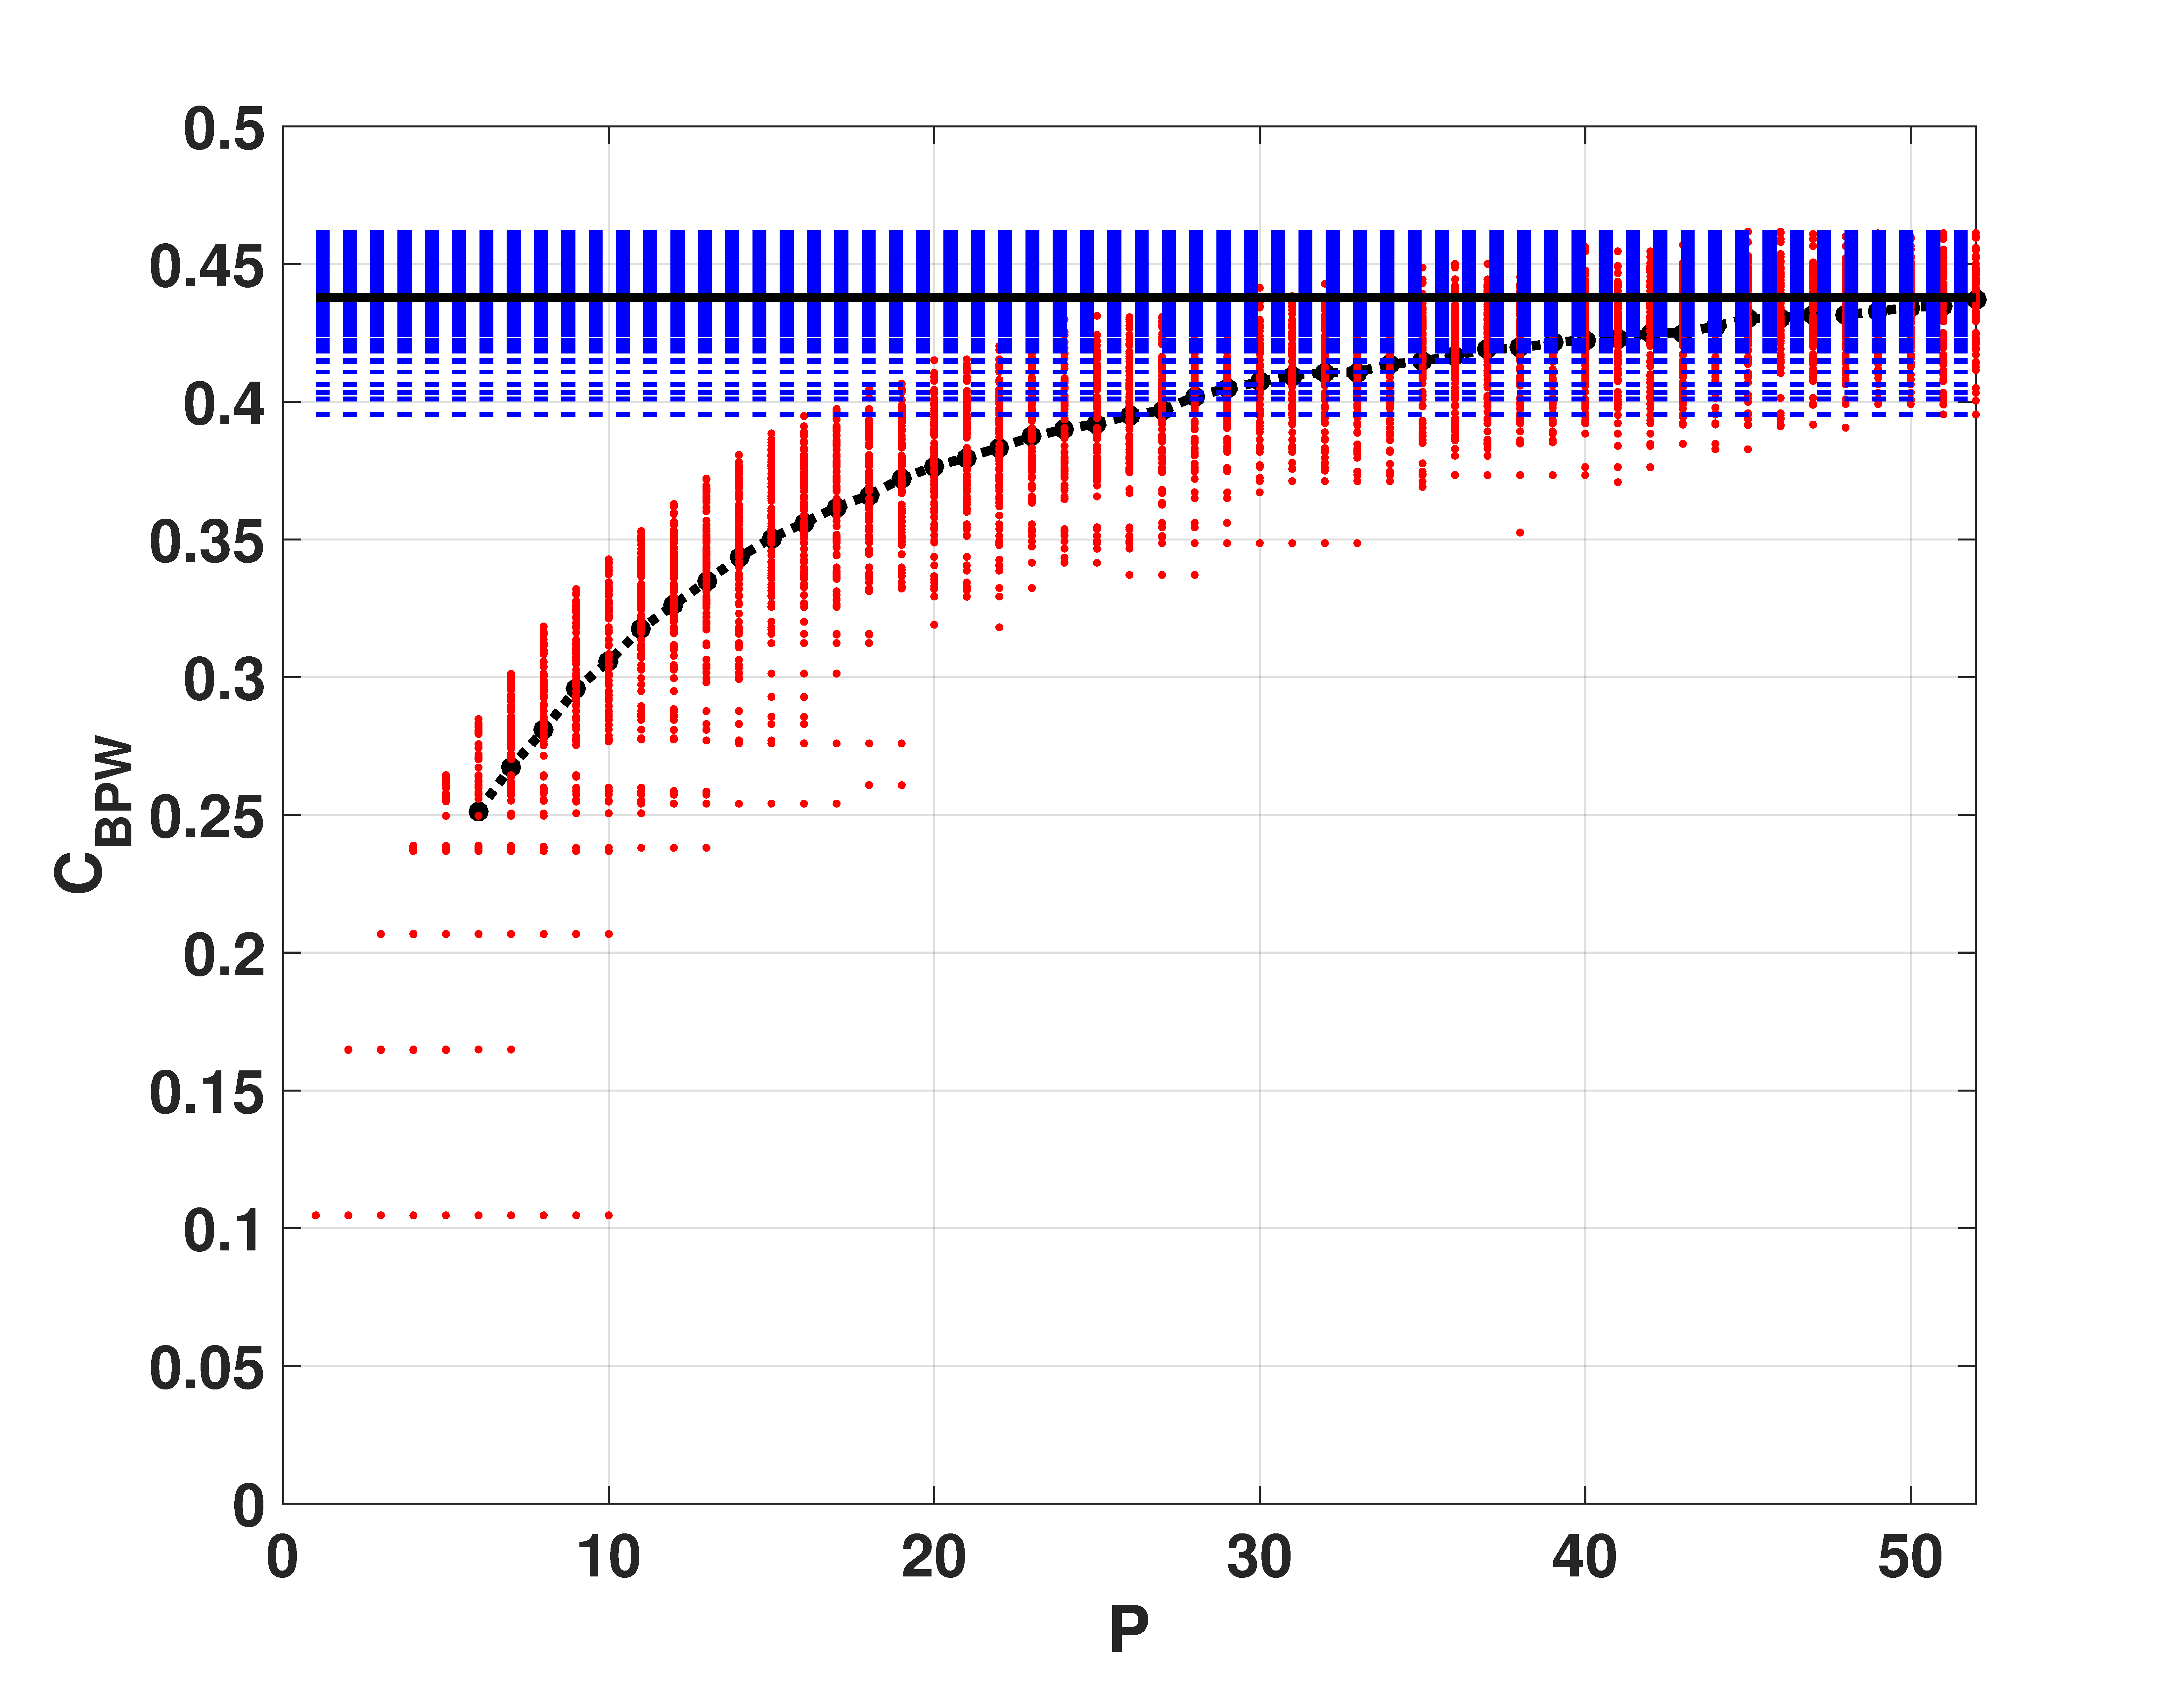
\includegraphics[width=.32\textwidth]{Cbpw_Tent}
	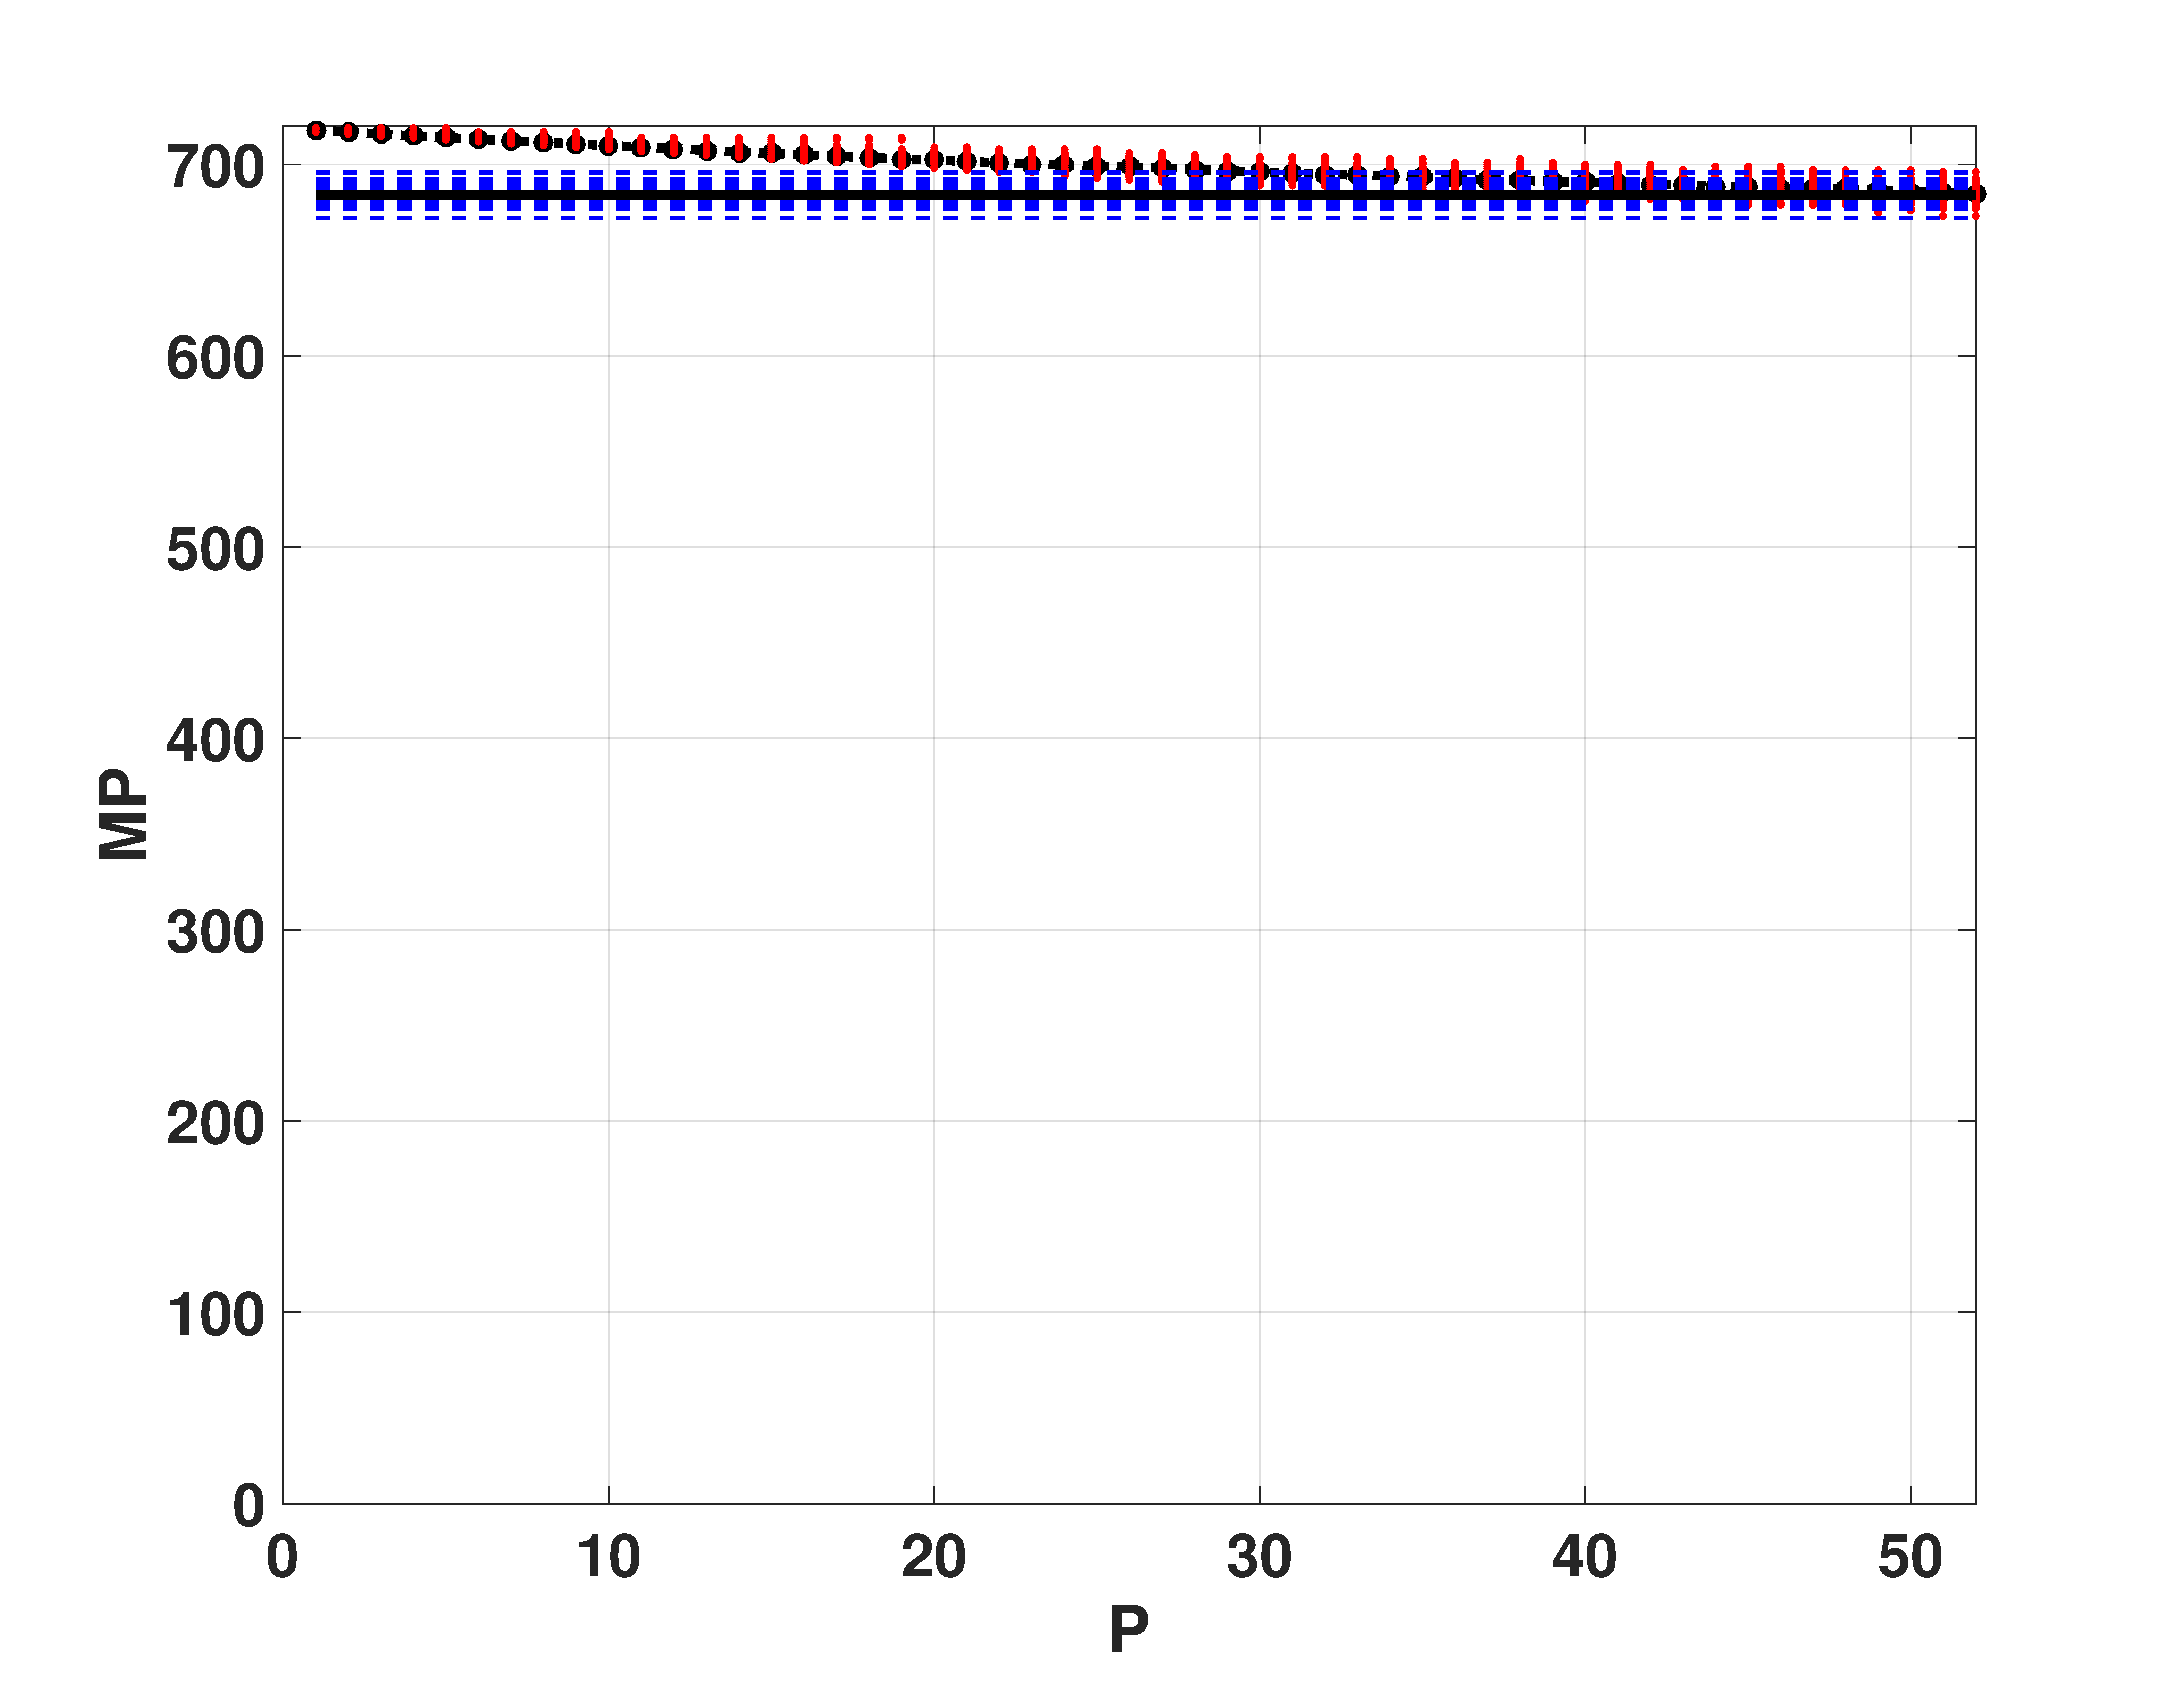
\includegraphics[width=.32\textwidth]{MP_Tent}
	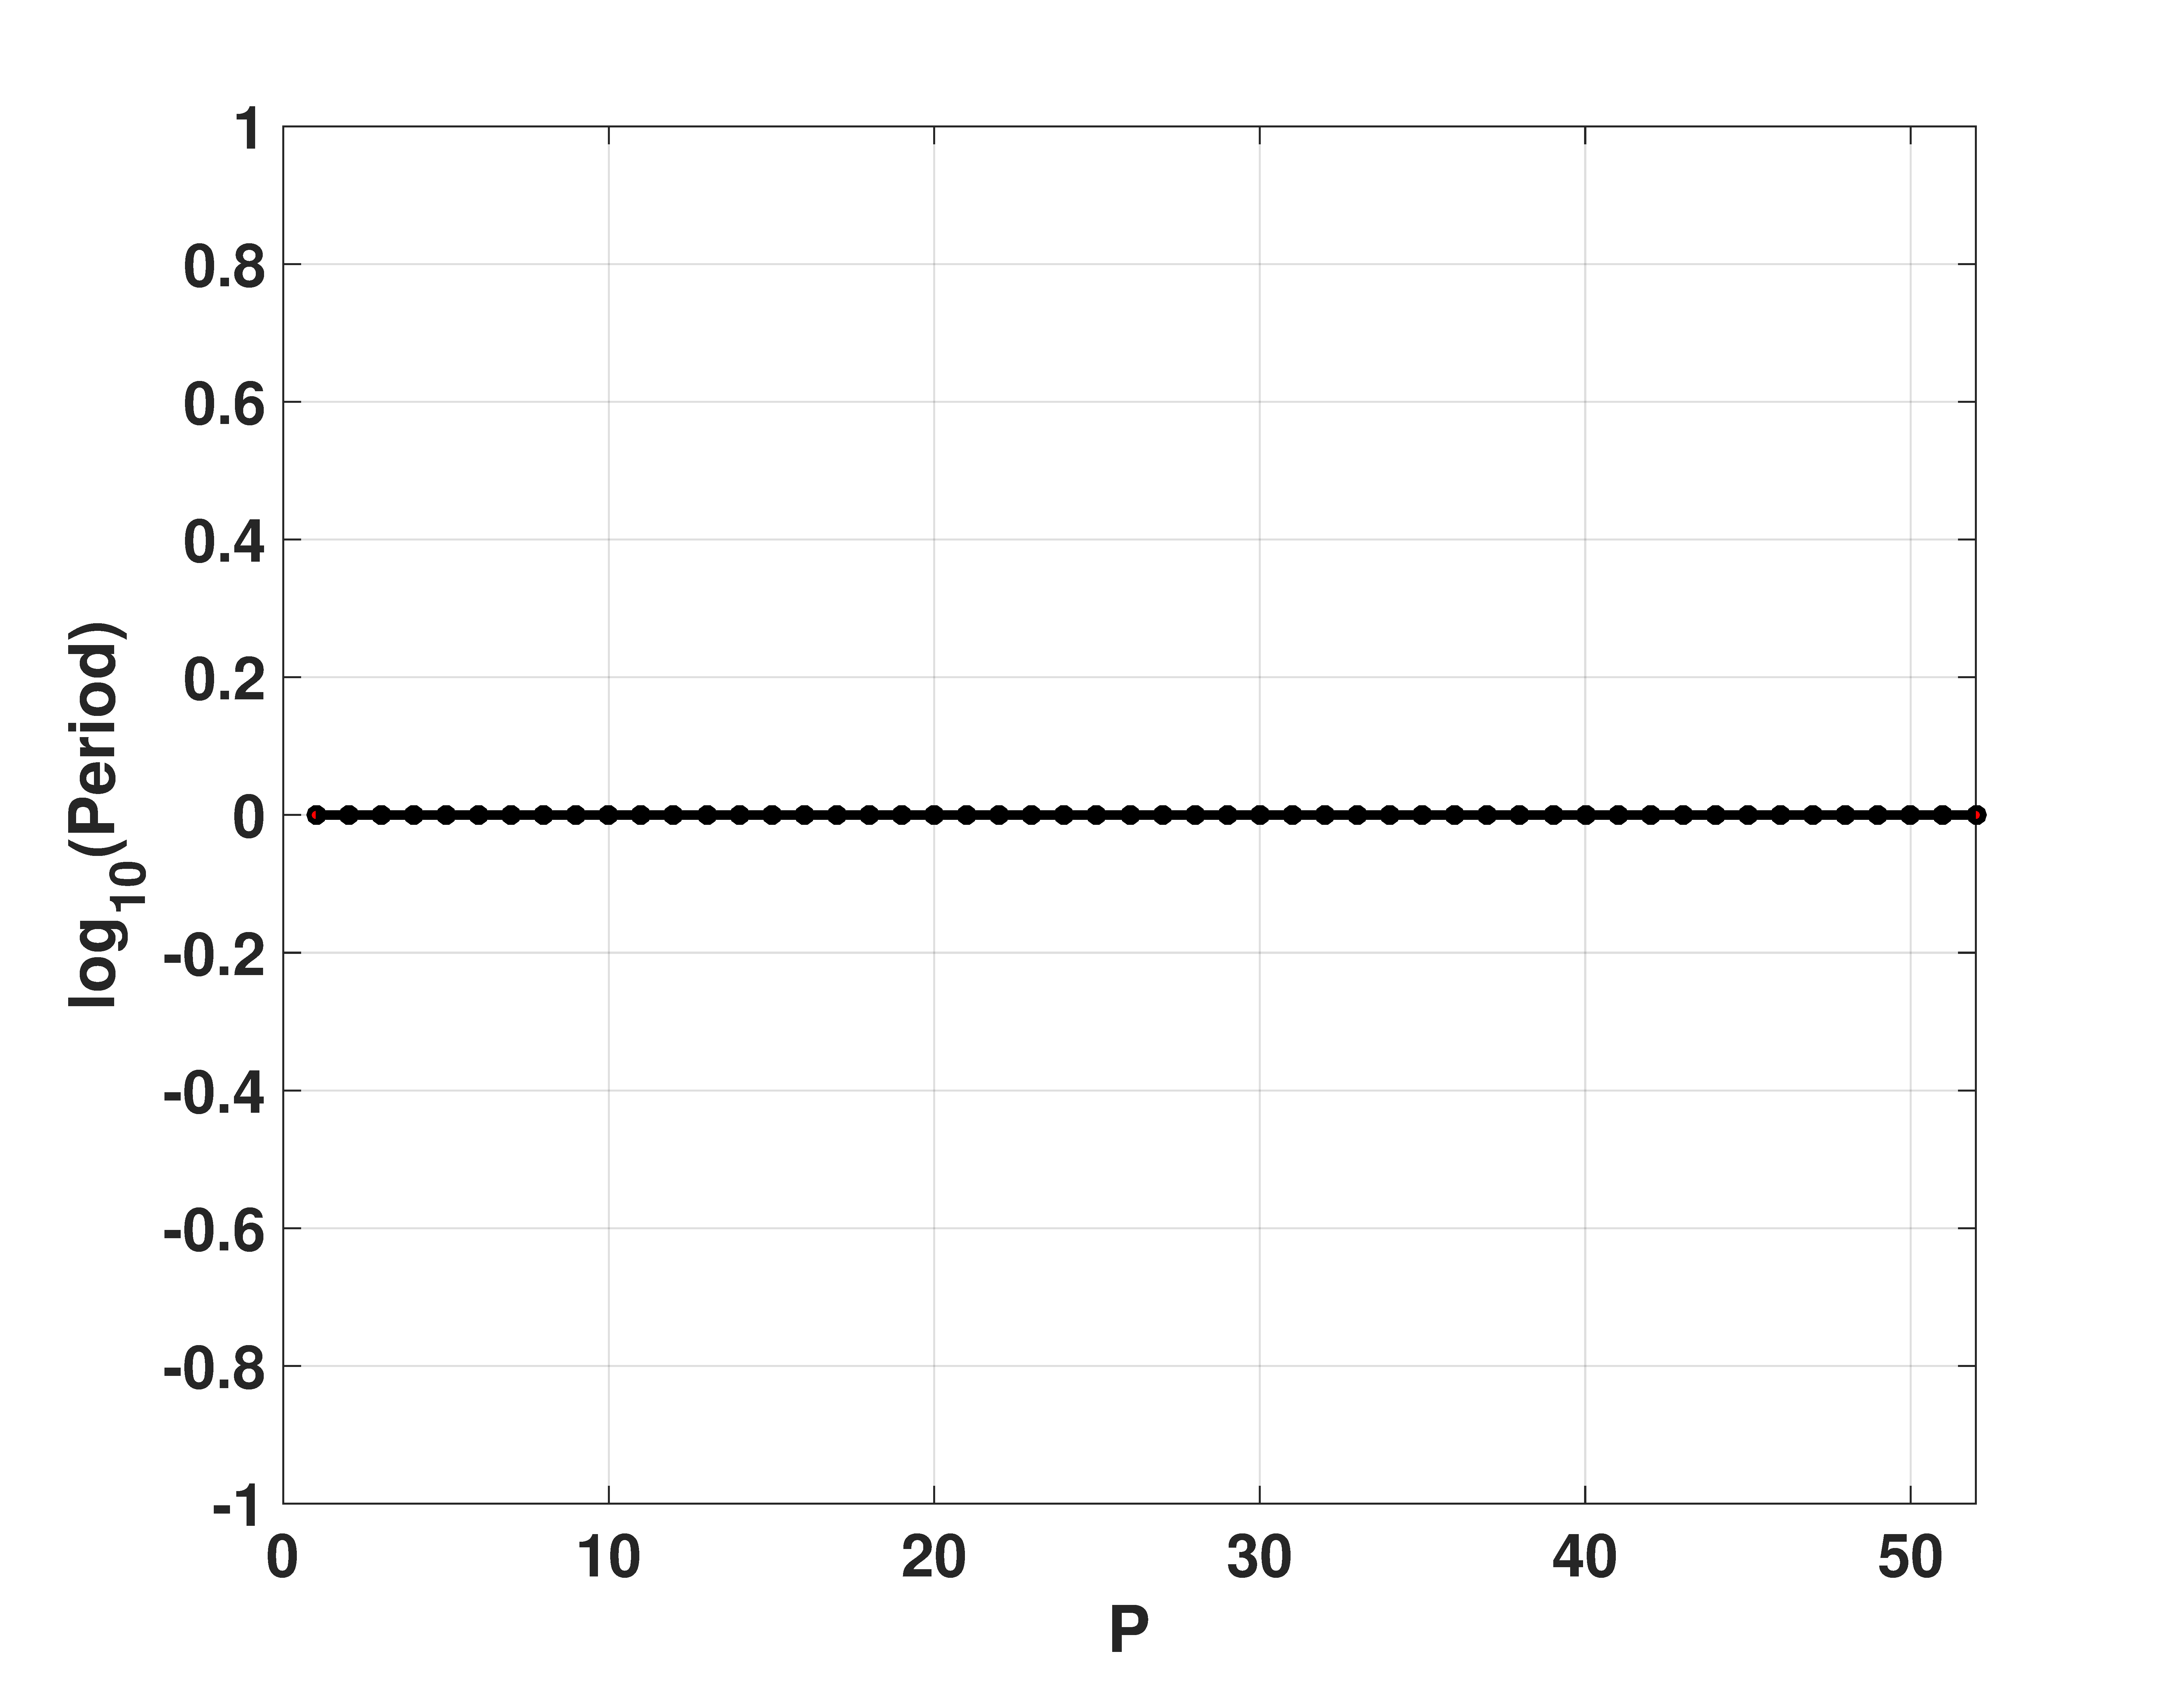
\includegraphics[width=.32\textwidth]{Period_Tent}
	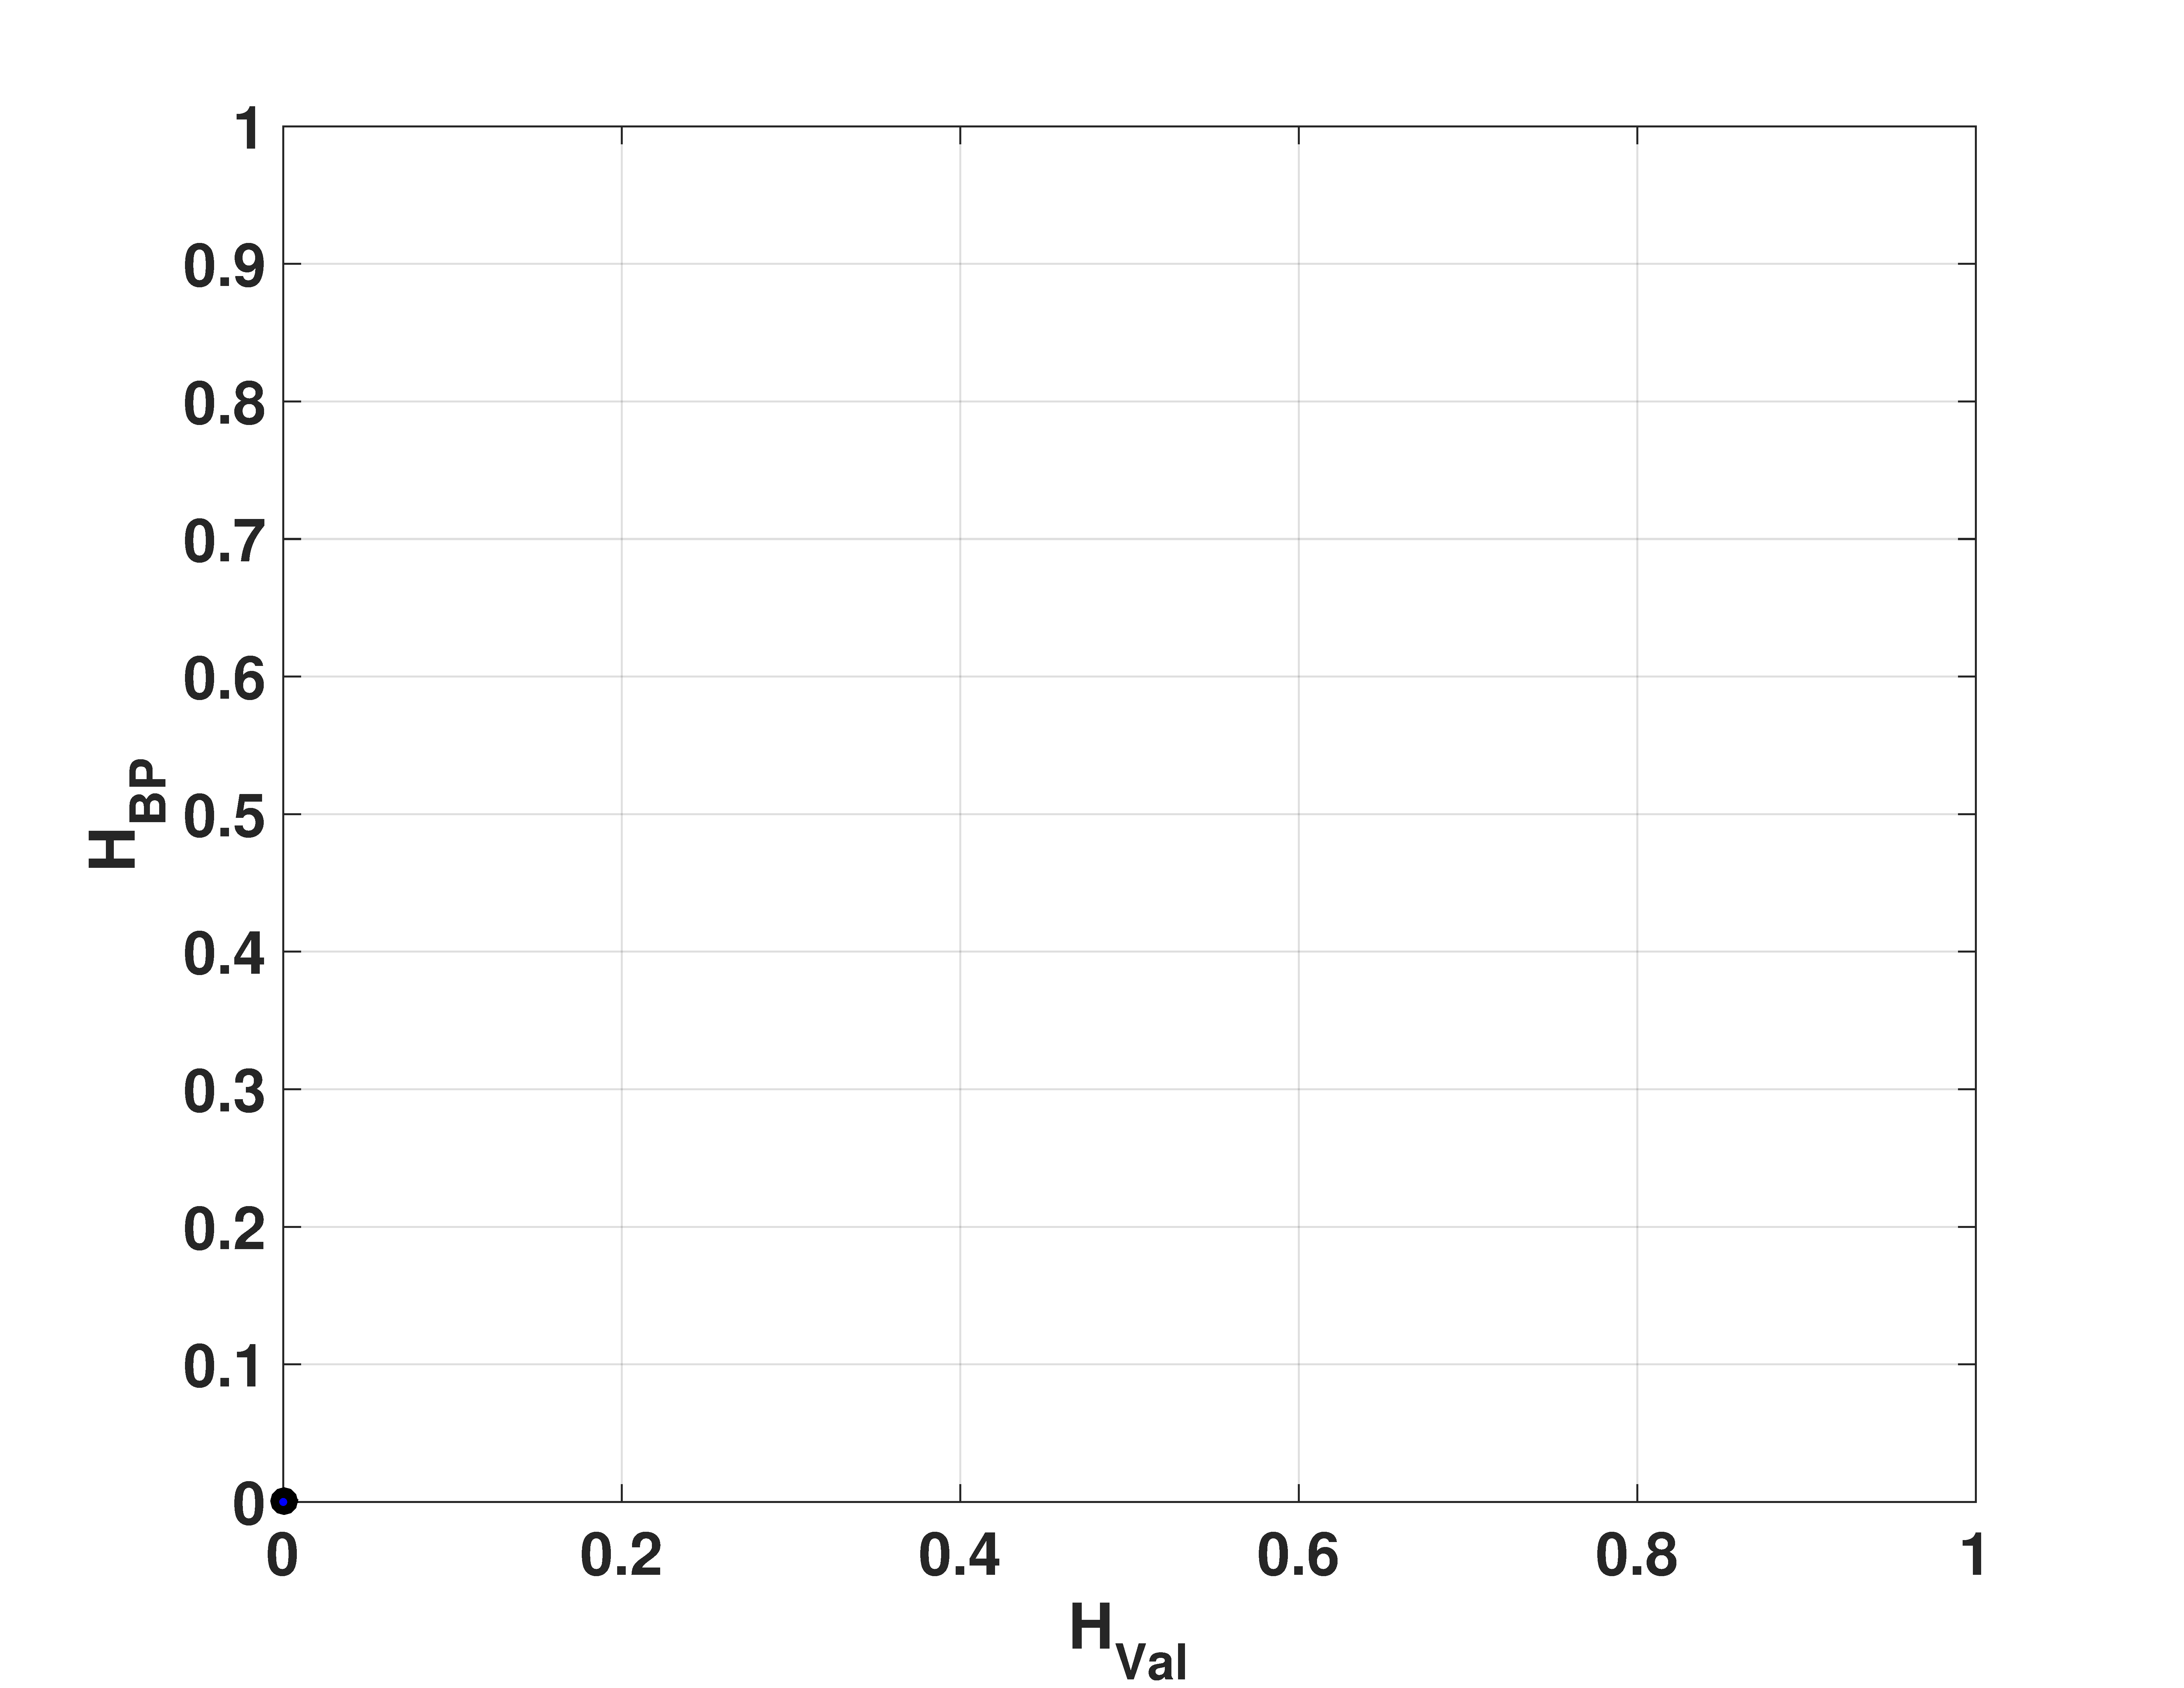
\includegraphics[width=.32\textwidth]{HbpHval_Tent}
	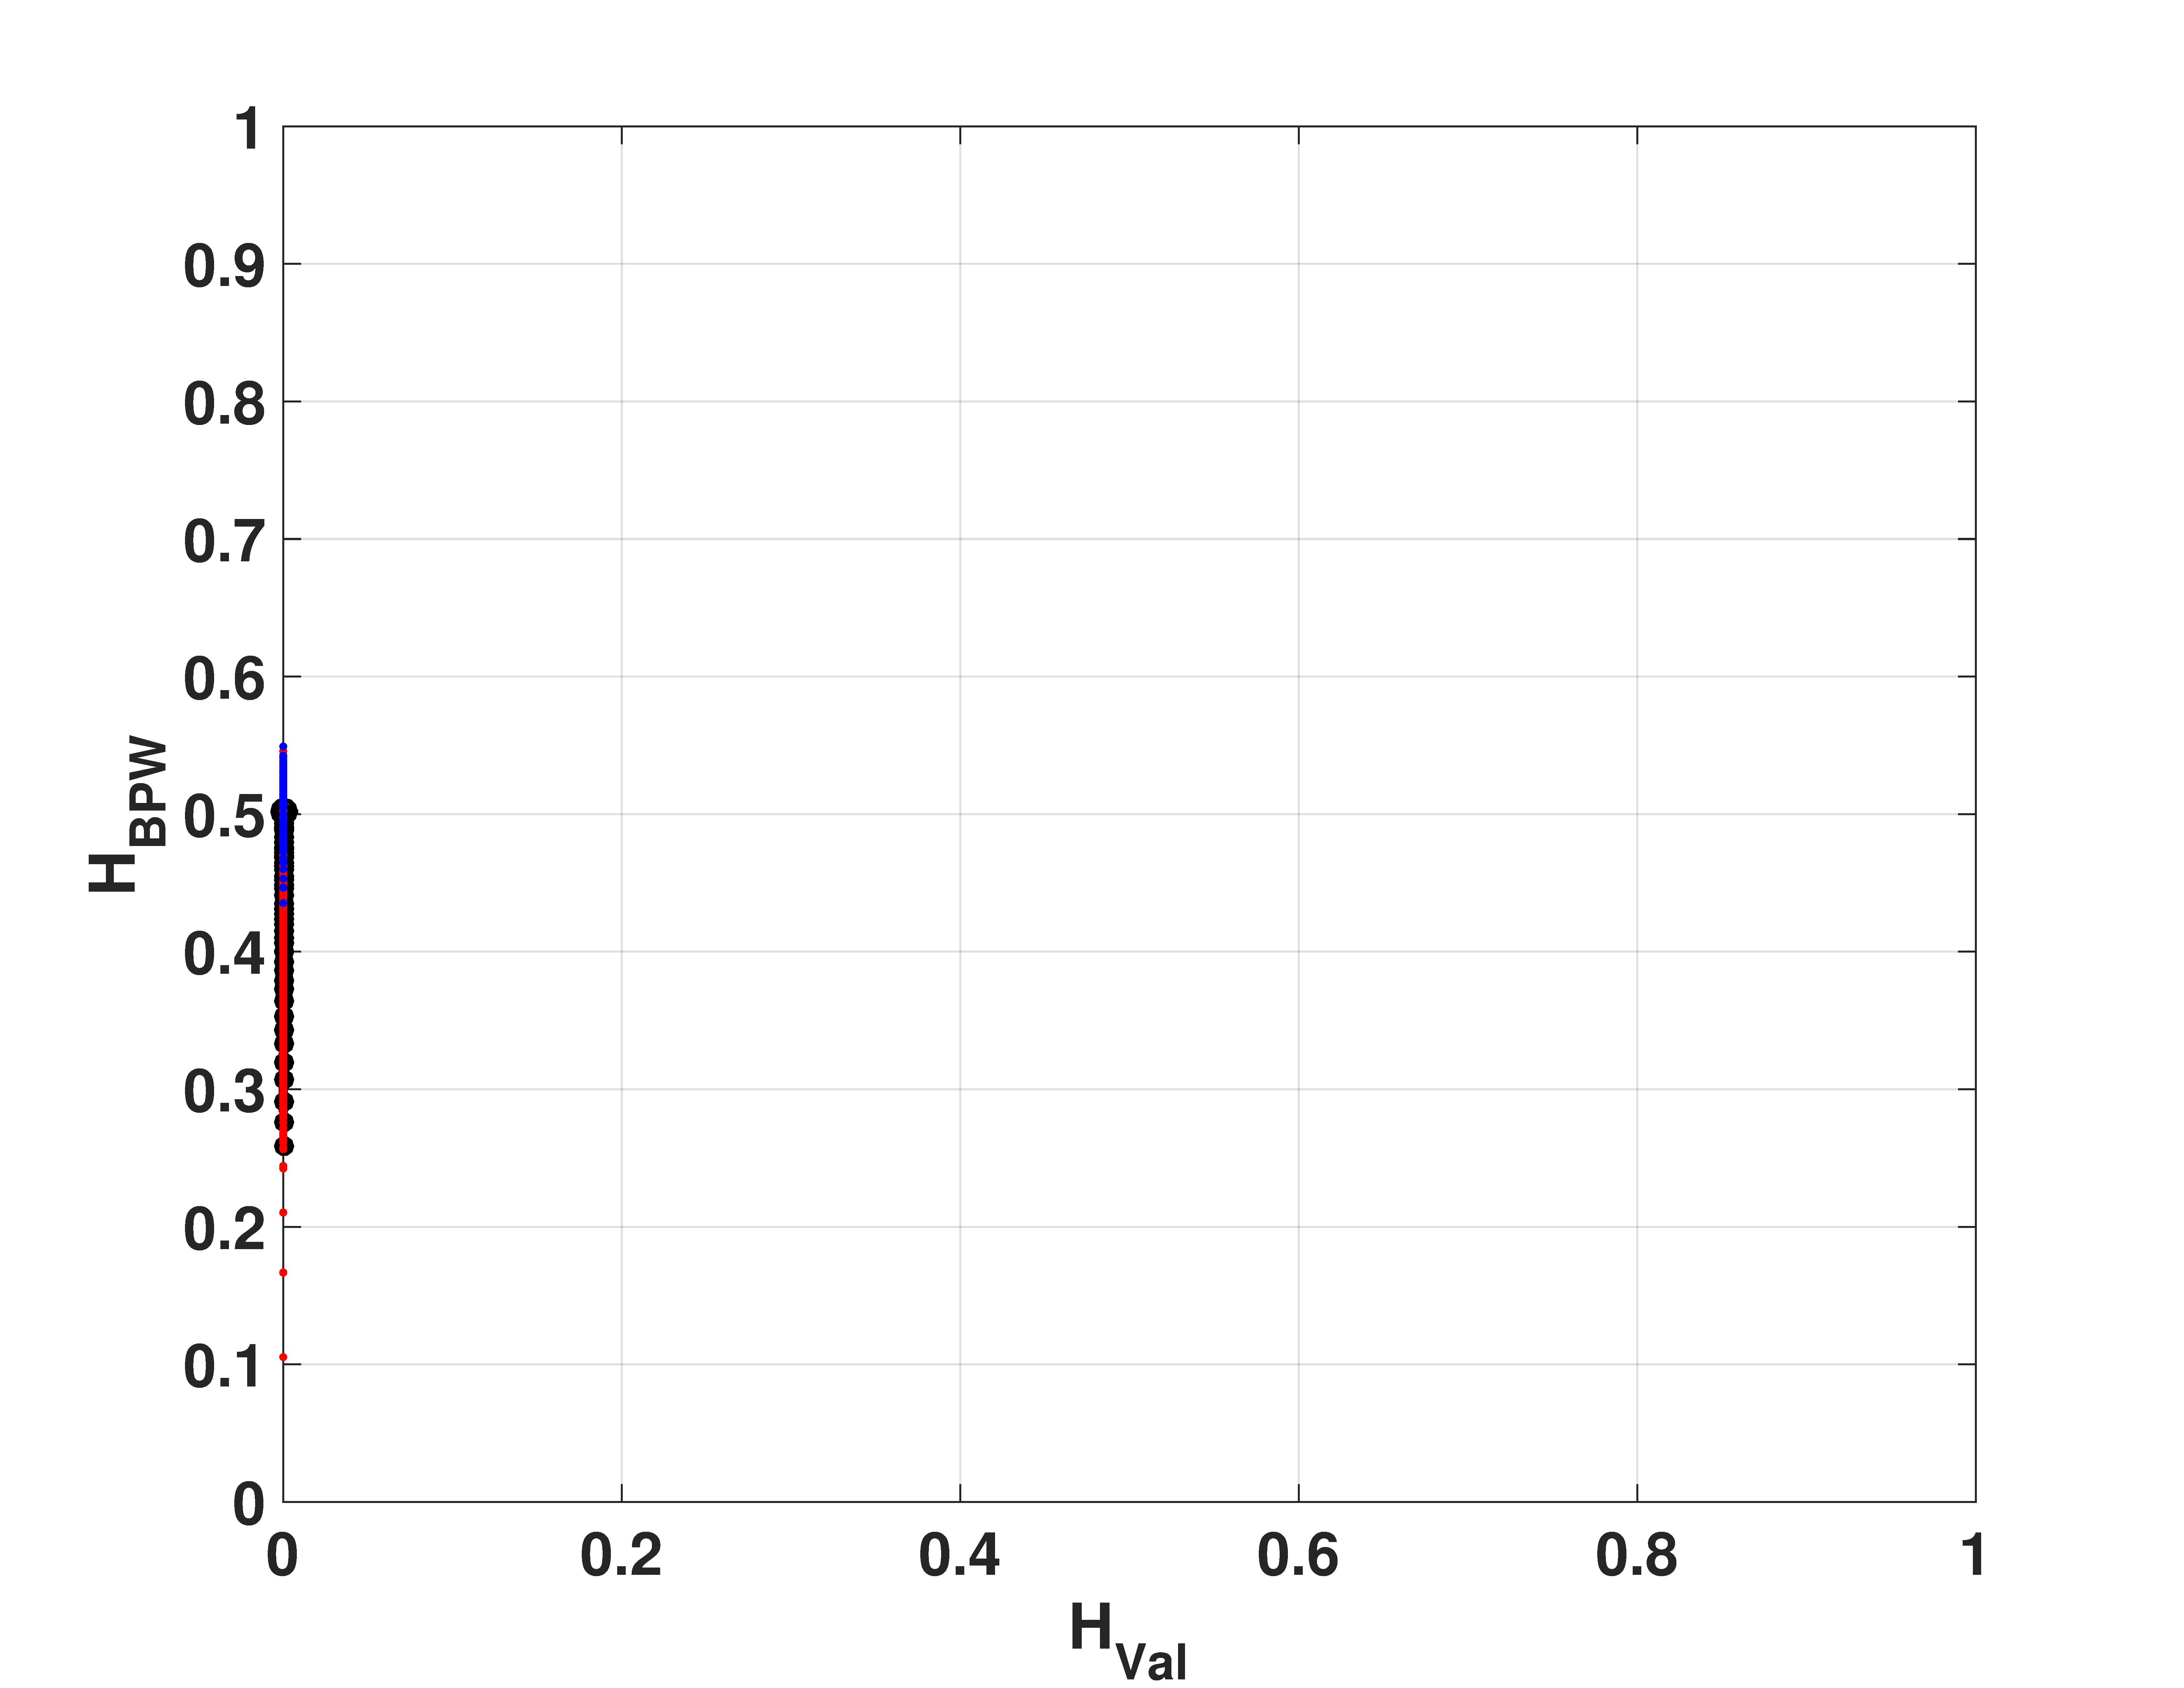
\includegraphics[width=.32\textwidth]{HbpwHval_Tent}
	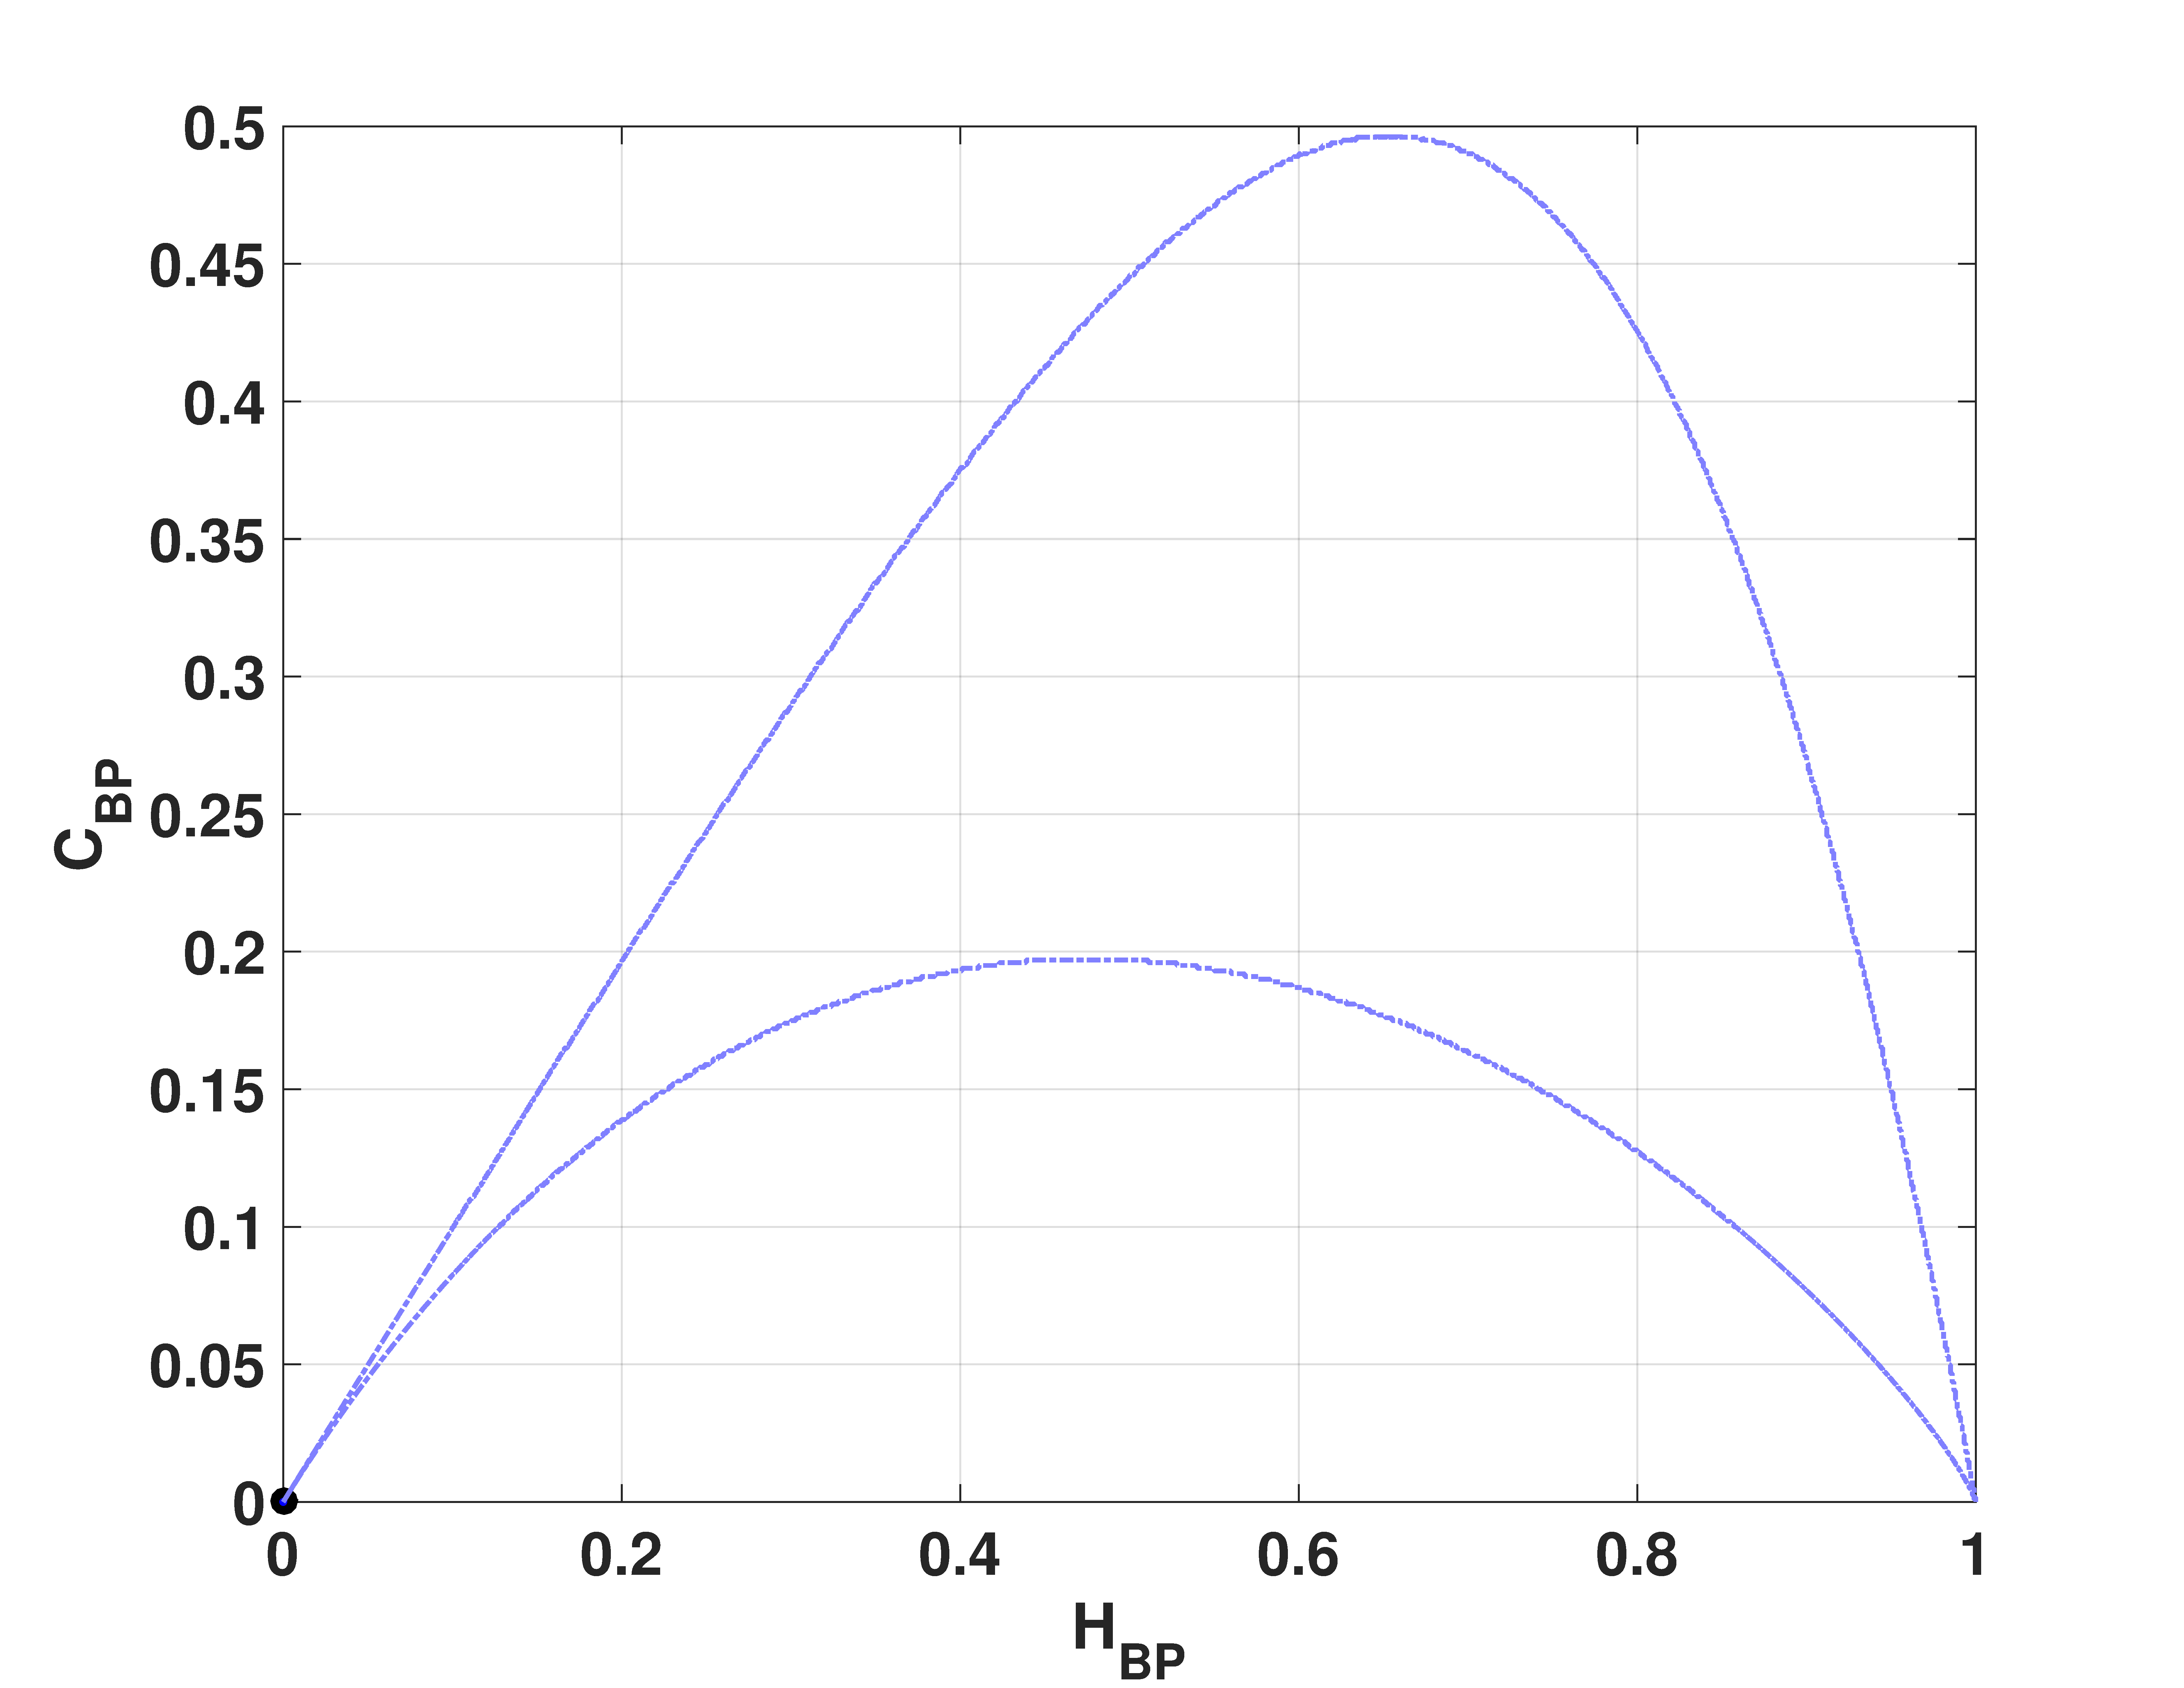
\includegraphics[width=.32\textwidth]{CbpHbp_Tent}
	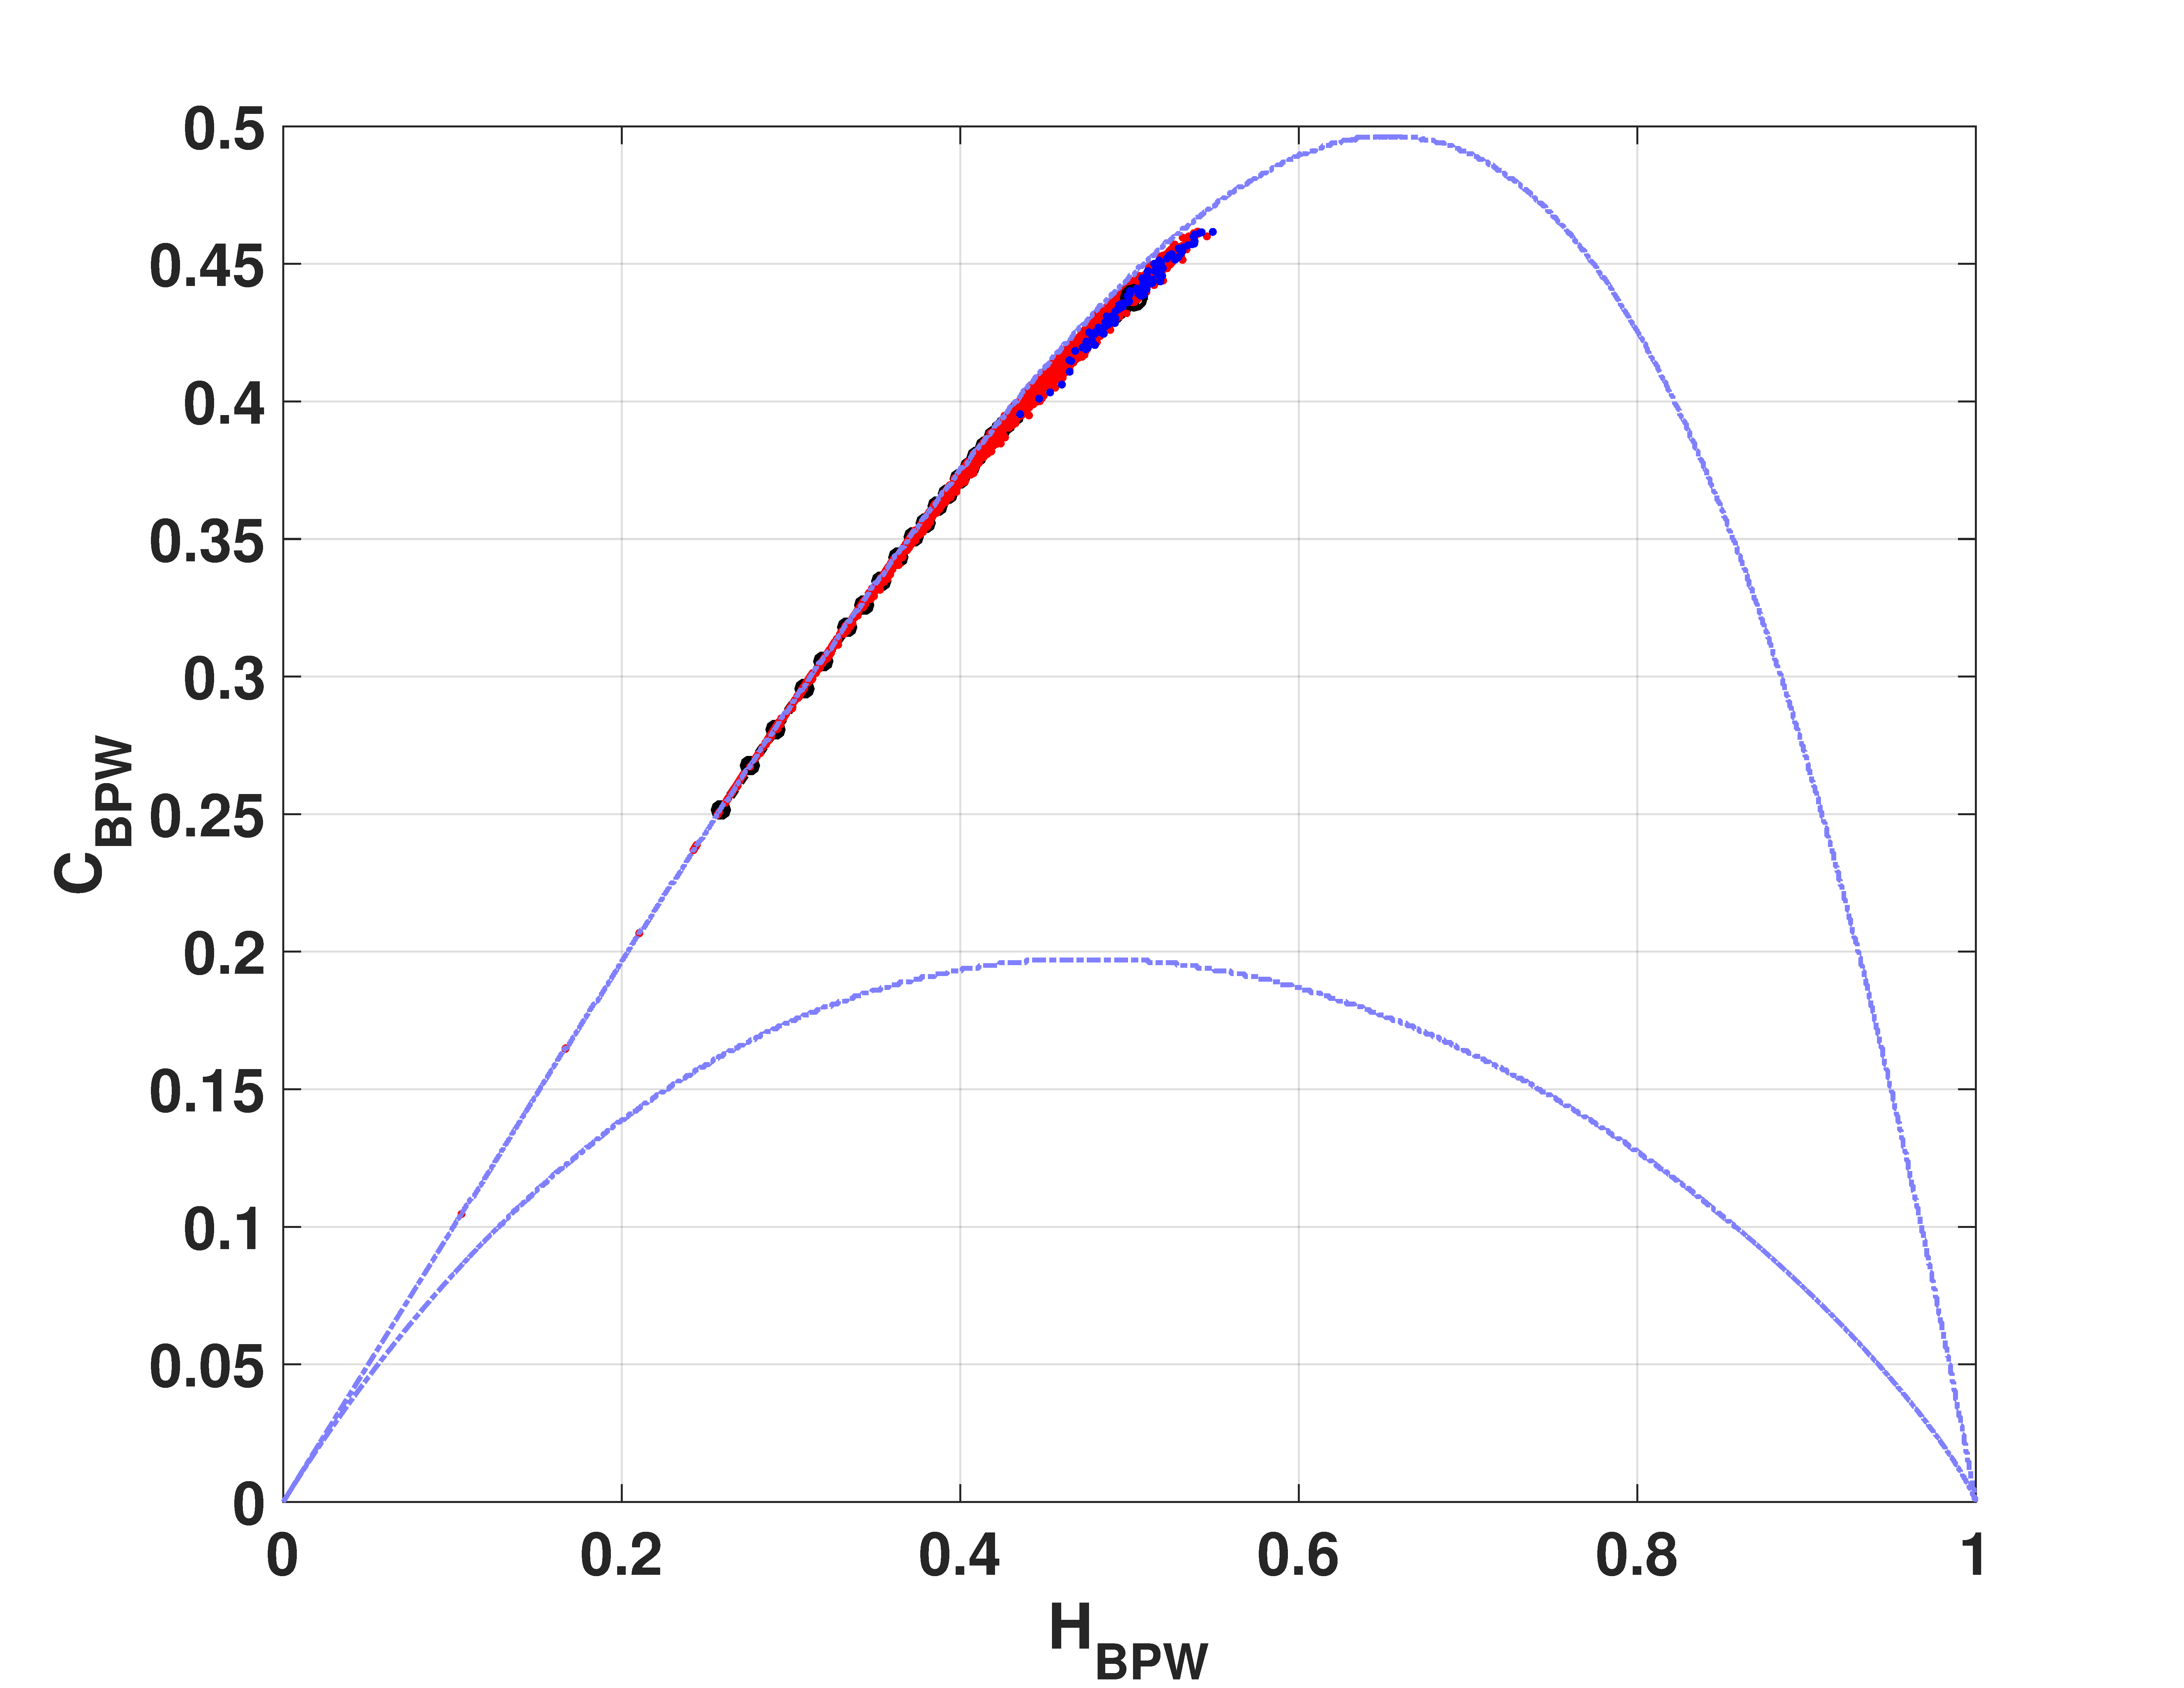
\includegraphics[width=.32\textwidth]{CbpwHbpw_Tent}
	\caption{Statistical properties of the TENT map using binary representation: (a) $H_{hist}$ vs $P$ (b) $H_{BP}$ vs $P$ (c) $C_{BP}$ vs $P$ (d) Number of missing ordering patterns $MP$ vs $P$. In Figures (a) to (d) dashed line correspond to floating point numbers. (e) representation in the $H_{hist},H_{BP}$ plane in the the binary numerical system.  The star represents the state for floating points numbers. (f) representation in the $H_{BP},C_{BP}$ plane.  The star represents the state for floating points numbers. (The star represents the state for floating points numbers). } \label{fig:tent}
\end{figure}
